% !TEX root = ../TUCthesis.tex
%****************************************************
\section{Implementierung}\label{ch:implementierung}
%****************************************************

% Schnittstellenrealisierung -> Interaktionsdiagramm

\subsection{Klassendiagramme}
%%%%%%%%%%%
%% Tests %%
%%%%%%%%%%%
\subsubsection{Tests.AbstractTestCase}
Die Abstrakte Klasse \verb|Tests.AbstractTestCase| hat die folgenden Schnittstellen:

\begin{figure}[H]
    \myfloatalign
    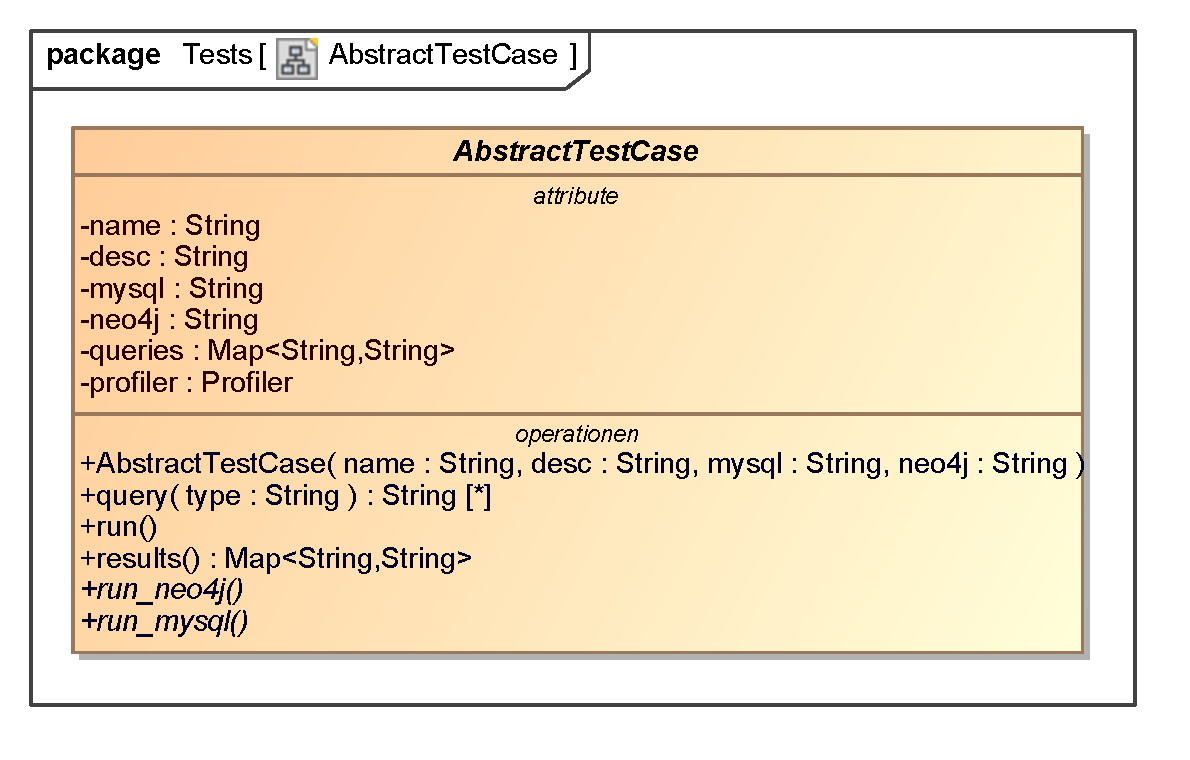
\includegraphics[width=0.85\textwidth]{gfx/MtGDeepAnalysis/AbstractTestCase.eps}
    \caption{Klassendiagramm Tests.AbstractTestCase}
    \label{fig:class:tests.abstracttestcase}
\end{figure}

\begin{description}
    \item[constructor(name, desc, mysql, neo4j)] \hfill \\
    Setzt den Namen \verb|name| und die Beschreibung \verb|desc| des Testfalls. Außerdem werden die Schlüssel \verb|mysql| und \verb|neo4j| festgelegt, welche für die Testergebnisse benutzt werden. Die Liste der Argumente befindet sich in \autoref{tab:tests.abstracttestcase.constructor}
    
    \item[query(type)] \hfill \\
    Gibt alle Abfragen für \verb|type = [mysql, neo4j]| die in dem Test ausgeführt werden zurück.
    
    \item[run()] \hfill \\
    Führt Test durch.
    
    \item[results()] \hfill \\
    Gibt aufgezeichnete Ergebnisse zurück nachdem der Test ausgeführt wurde.
    
    \item[run\_neo4j()] \hfill \\
    Testfall für Neo4j-Datenbank.
    
    \item[run\_mysql()] \hfill \\
    Testfall für MySQL-Datenbank.
\end{description}


\begin{table}[h]
    \caption{Tests.AbstractTestCase::constructor(name : string, desc : string, mysql : string, neo4j : string)} 
    \myfloatalign
    \begin{tabularx}{\textwidth}{lX}
        \toprule 
        \tableheadline{Eingabe} & \tableheadline{Beschreibung} \\ 
        \midrule 
        \verb|name : string| & Name des Testfalls \\
        \verb|desc : string| & Beschreibung des Testfalls \\
        \verb|mysql : string| & Schlüssel für MySQL-Testergebnisse \\
        \verb|neo4j : string| & Schlüssel für Neo4j-Testergebnisse \\
        \bottomrule 
    \end{tabularx}
    \label{tab:tests.abstracttestcase.constructor}
\end{table}

\subsubsection{Tests.CardTestcase}
Die Abstrakte Klasse \verb|Tests.CardTestcase| hat die folgenden Schnittstellen:

\begin{figure}[H]
    \myfloatalign
    \includegraphics[width=0.65\textwidth]{gfx/MtGDeepAnalysis/CardTestcase.eps}
    \caption{Klassendiagramm Tests.CardTestcase}
    \label{fig:class:tests.CardTestcase}
\end{figure}

\begin{description}
    \item[init\_queries()] \hfill \\
    Fügt Standardabfragen zu \verb|queries| hinzu, welche für die Kartentests gebraucht werden
        
    \item[run\_neo4j()] \hfill \\
    Cypher-Abfragen ausführen und Karten in Datenstruktur \verb|Transformations.Cards| überführen
    
    \item[run\_mysql()] \hfill \\
    SQL-Abfragen ausführen und Karten in Datenstruktur \verb|Transformations.Cards| überführen
\end{description}

\subsubsection{Tests.Manager}
Die Klasse \verb|Tests.Manager| hat die folgenden Schnittstellen:

\begin{figure}[H]
    \myfloatalign
    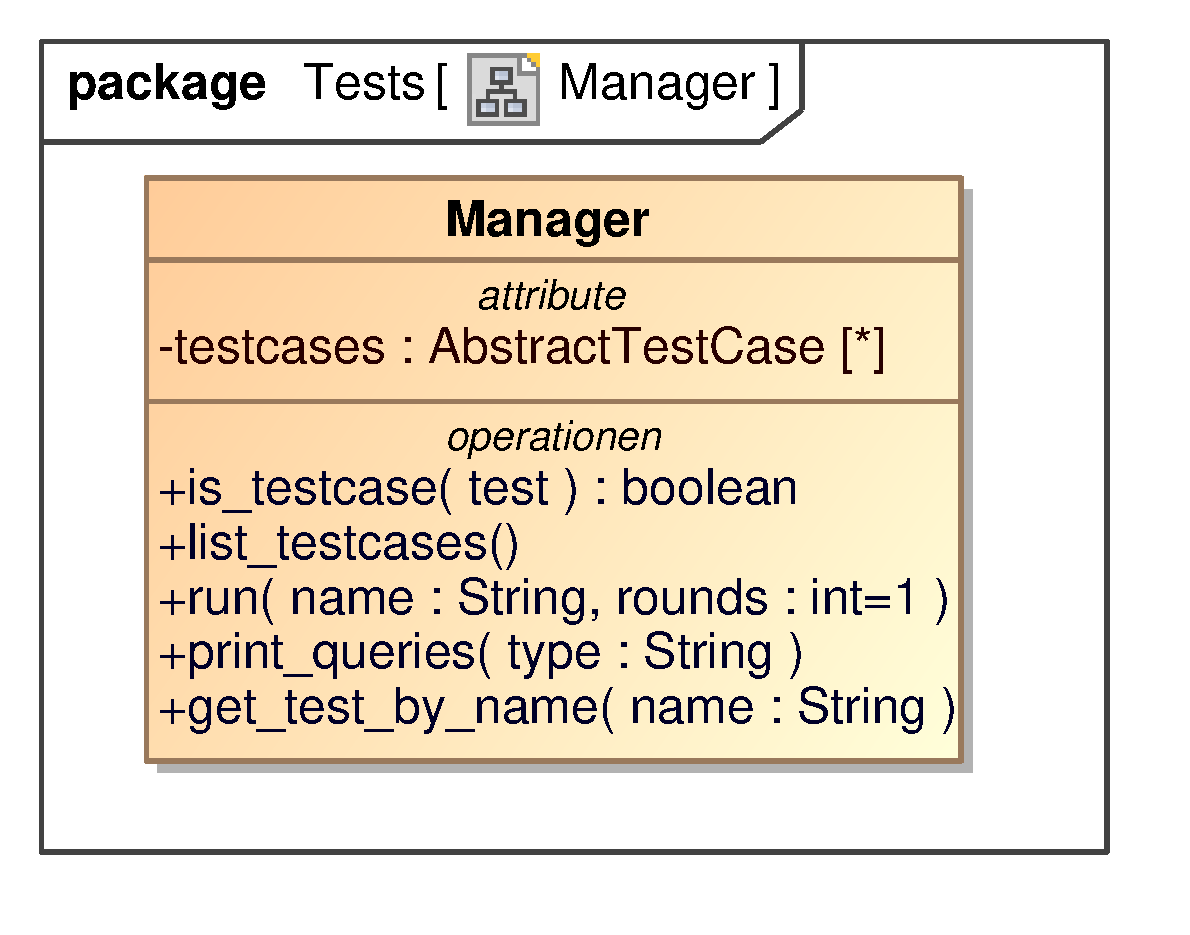
\includegraphics[width=0.65\textwidth]{gfx/MtGDeepAnalysis/Manager.eps}
    \caption{Klassendiagramm Tests.Manager}
    \label{fig:class:tests.manager}
\end{figure}

\begin{description}
    \item[Manager()] \hfill \\
    Lädt alle Testfälle und speichert diese in \verb|testcases|
    
    \item[is\_testcase(test)] \hfill \\
    Prüft ob ein Objekt \verb|test| ein Testfall ist, das heißt von \verb|Tests.AbstractTestCase| abgeleitet ist.
    
    \item[list\_testcases()] \hfill \\
    Gibt eine Liste der verfügbaren Tests in \verb|testcases| aus
    
    \item[run(name, rounds)] \hfill \\
    Führt den Testfall \verb|name| \verb|rounds|-mal hintereinander aus
    
    \item[print\_queries(name)] \hfill \\
    Gibt alle Abfragen des Testfalls \verb|name| aus.
    
    \item[get\_test\_by\_name(name)] \hfill \\
    Gibt den Testfall \verb|name| zurück, sofern dieser sich in \verb|testcases| befindet
\end{description}

\subsubsection{Tests.Testcase\_ComplexCardSearch}
Die Klasse \verb|Tests.Testcase_ComplexCardSearch| hat die folgenden Schnittstellen:

\begin{figure}[H]
    \myfloatalign
    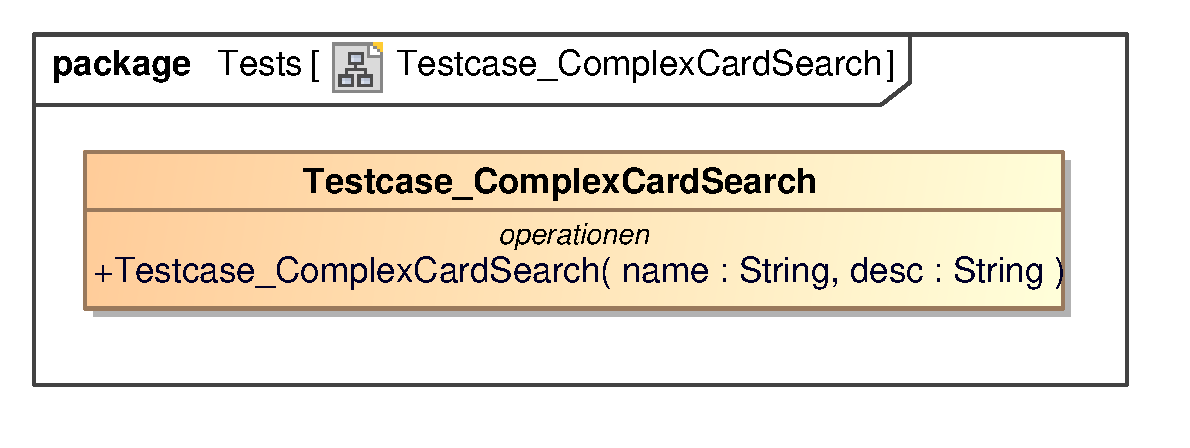
\includegraphics[width=0.75\textwidth]{gfx/MtGDeepAnalysis/Testcase_ComplexCardSearch.eps}
    \caption{Klassendiagramm Tests.Testcase\_ComplexCardSearch}
    \label{fig:class:tests.Testcase_ComplexCardSearch}
\end{figure}

\begin{description}
    \item[Testcase\_ComplexCardSearch(name, desc)] \hfill \\
    Fügt Abfragen des Testfalls zu \verb|queries| hinzu
\end{description}

\subsubsection{Tests.Testcase\_Matchup}
Die Klasse \verb|Tests.Testcase_Matchup| hat die folgenden Schnittstellen:

\begin{figure}[H]
    \myfloatalign
    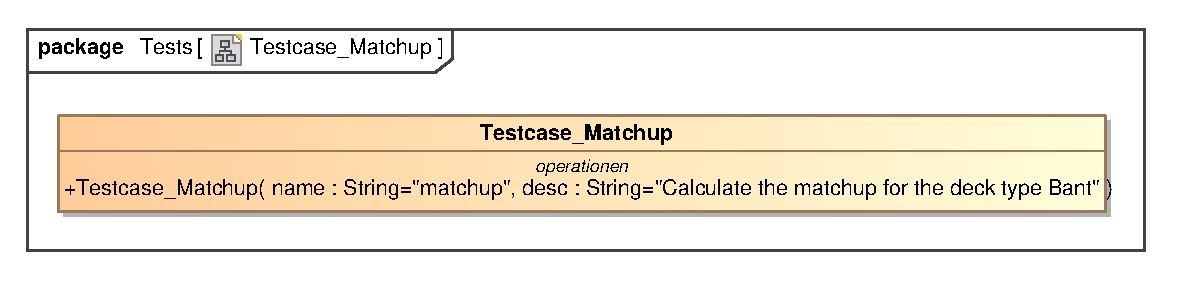
\includegraphics[width=0.75\textwidth]{gfx/MtGDeepAnalysis/Testcase_Matchup.eps}
    \caption{Klassendiagramm Tests.Testcase\_Matchup}
    \label{fig:class:tests.Testcase_Matchup}
\end{figure}

\begin{description}
    \item[Testcase\_Matchup(name, desc)] \hfill \\
    Fügt Abfragen des Testfalls zu \verb|queries| hinzu
\end{description}

\subsubsection{Tests.Testcase\_SimpleArtistCardSearch}
Die Klasse \verb|Tests.Testcase_SimpleArtistCardSearch| hat die folgenden Schnittstellen:

\begin{figure}[H]
    \myfloatalign
    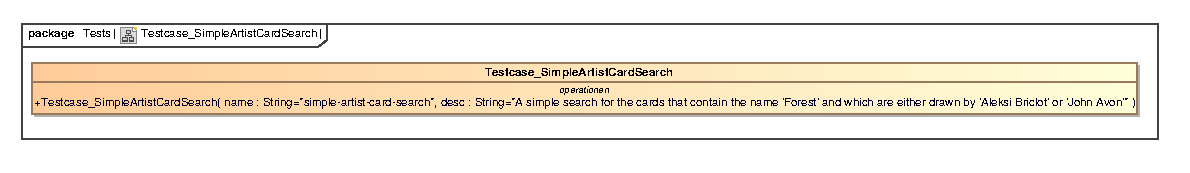
\includegraphics[width=0.75\textwidth]{gfx/MtGDeepAnalysis/Testcase_SimpleArtistCardSearch.eps}
    \caption{Klassendiagramm Tests.Testcase\_SimpleArtistCardSearch}
    \label{fig:class:tests.Testcase_SimpleArtistCardSearch}
\end{figure}

\begin{description}
    \item[Testcase\_SimpleArtistCardSearch(name, desc)] \hfill \\
    Fügt Abfragen des Testfalls zu \verb|queries| hinzu
\end{description}

\subsubsection{Tests.Testcase\_SimpleKeywordAbilitySearch}
Die Klasse \verb|Tests.Testcase_SimpleKeywordAbilitySearch| hat die folgenden Schnittstellen:

\begin{figure}[H]
    \myfloatalign
    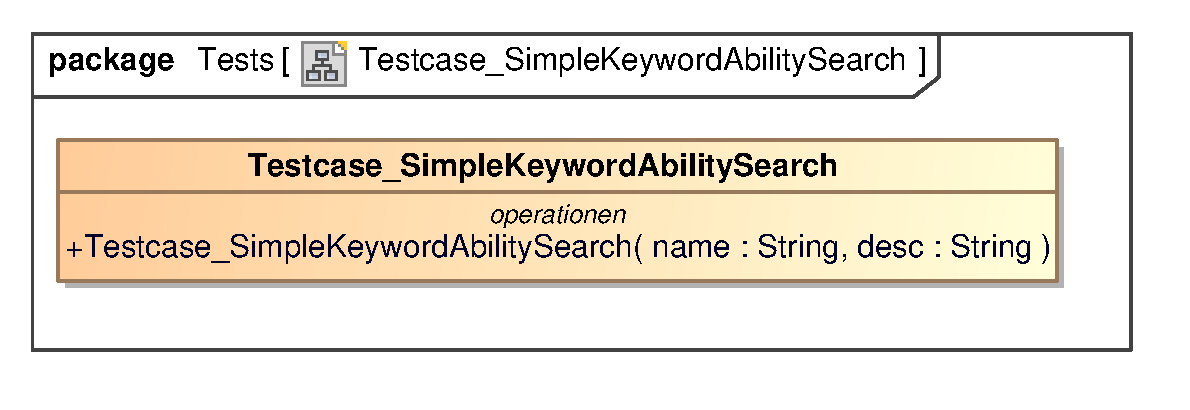
\includegraphics[width=0.75\textwidth]{gfx/MtGDeepAnalysis/Testcase_SimpleKeywordAbilitySearch.eps}
    \caption{Klassendiagramm Tests.Testcase\_SimpleKeywordAbilitySearch}
    \label{fig:class:tests.Testcase_SimpleKeywordAbilitySearch}
\end{figure}

\begin{description}
    \item[Testcase\_SimpleKeywordAbilitySearch(name, desc)] \hfill \\
    Fügt Abfragen des Testfalls zu \verb|queries| hinzu
\end{description}

\subsubsection{Tests.Testcase\_TopTenDecks}
Die Klasse \verb|Tests.Testcase_TopTenDecks| hat die folgenden Schnittstellen:

\begin{figure}[H]
    \myfloatalign
    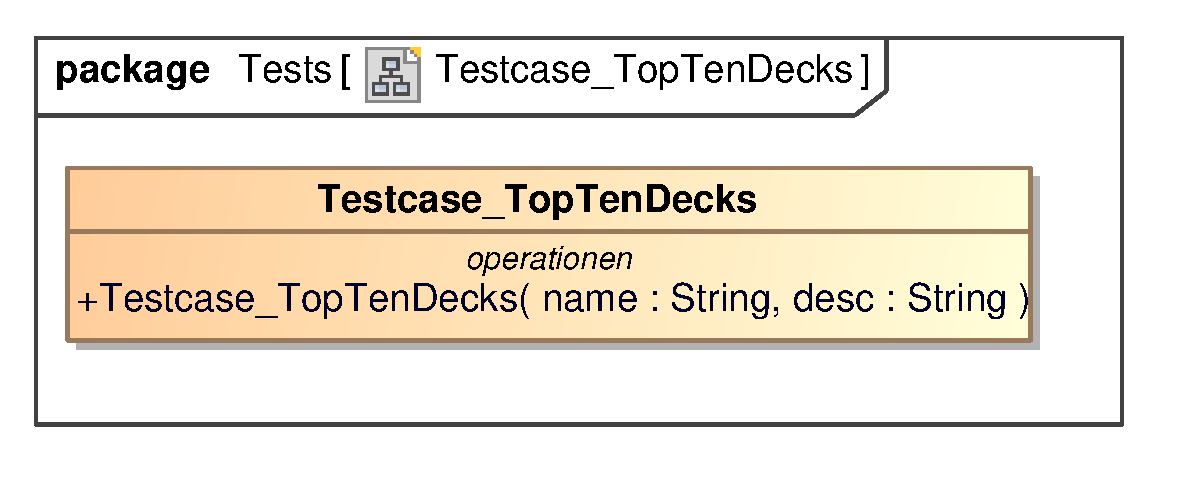
\includegraphics[width=0.75\textwidth]{gfx/MtGDeepAnalysis/Testcase_TopTenDecks.eps}
    \caption{Klassendiagramm Tests.Testcase\_TopTenDecks}
    \label{fig:class:tests.Testcase_TopTenDecks}
\end{figure}

\begin{description}
    \item[Testcase\_TopTenDecks(name, desc)] \hfill \\
    Fügt Abfragen des Testfalls zu \verb|queries| hinzu
\end{description}

%%%%%%%%%%%%%%%%
%% Foundation %%
%%%%%%%%%%%%%%%%
\subsubsection{Foundation.Config}
Die Klasse \verb|Foundation.Config| hat die folgenden Schnittstellen:

\begin{figure}[H]
    \myfloatalign
    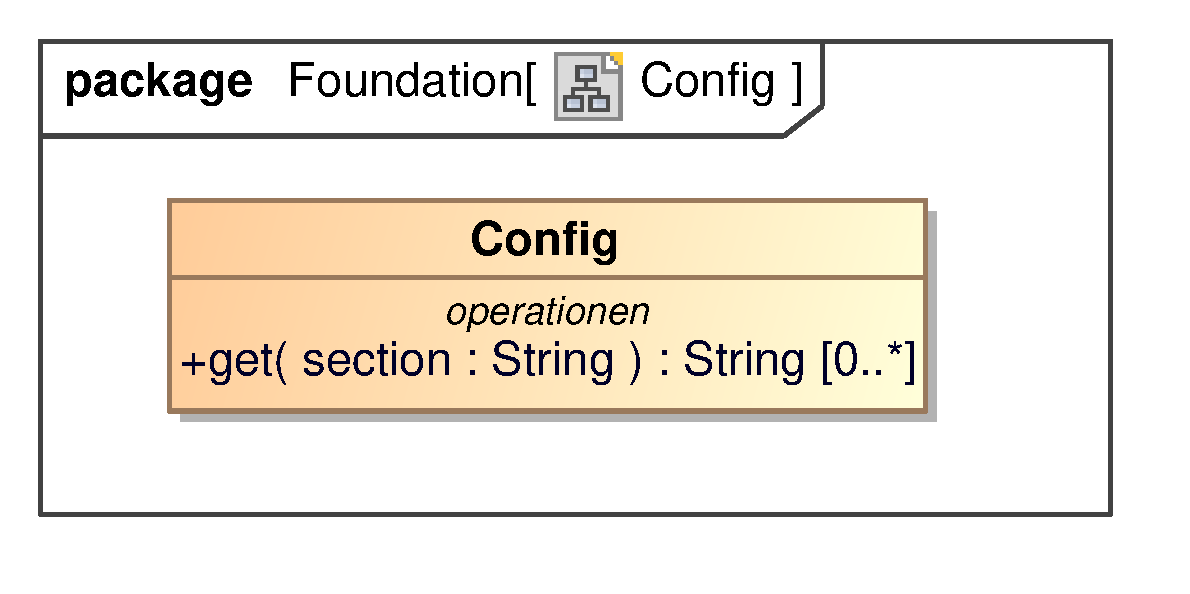
\includegraphics[width=0.75\textwidth]{gfx/MtGDeepAnalysis/Config.eps}
    \caption{Klassendiagramm Foundation.Config}
    \label{fig:class:foundation.config}
\end{figure}

\begin{description}
    \item[Config()] \hfill \\
    Lädt die Konfigurationsdatei Datei \verb|config.ini|
    
    \item[get(section)] \hfill \\
    Gibt einen Konfigurationsabschnitt \verb|section| als \verb|string[]| aus der Datei \verb|config.ini| zurück
\end{description}


\subsubsection{Foundation.Database}
Die Klasse \verb|Foundation.Database| hat die folgenden Schnittstellen:

\begin{figure}[H]
    \myfloatalign
    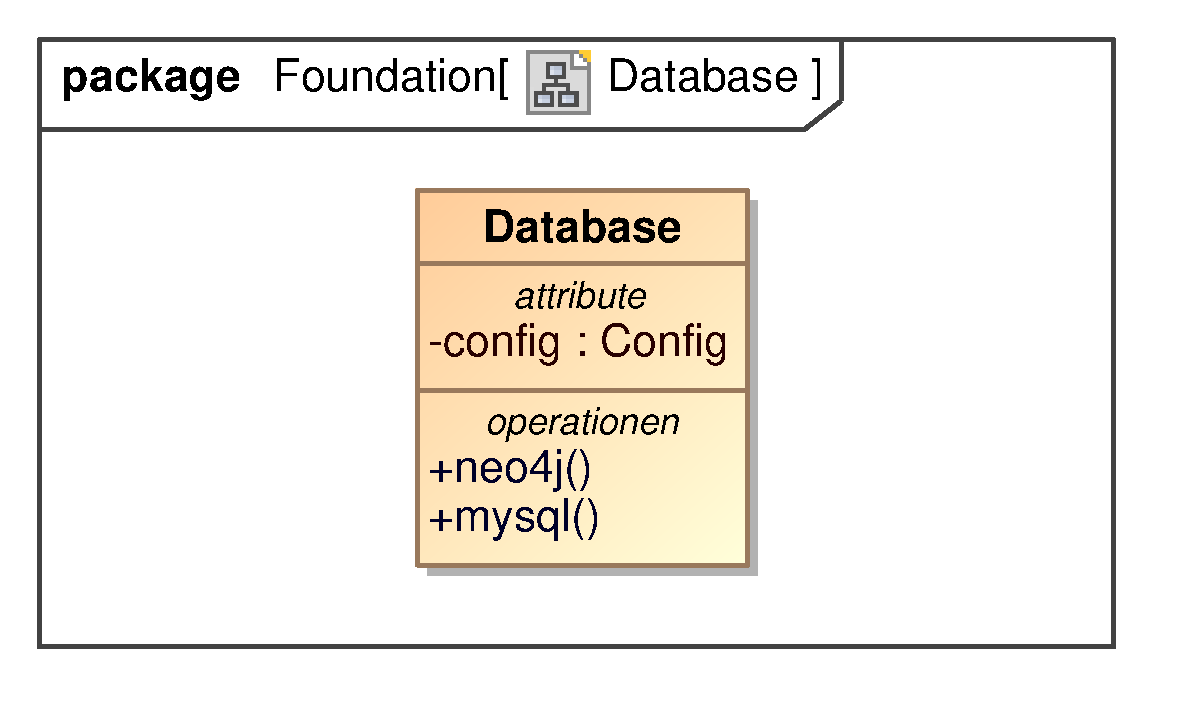
\includegraphics[width=0.75\textwidth]{gfx/MtGDeepAnalysis/Database.eps}
    \caption{Klassendiagramm Foundation.Database}
    \label{fig:class:foundation.database}
\end{figure}

\begin{description}
    \item[Database()] \hfill \\
    Erstellt eine neue \verb|Foundation.Config| Instanz und speichert diese in \verb|config|.
    
    \item[neo4j()] \hfill \\
    Gibt eine neue Neo4j Datenbank-Instanz zurück.
    
    \item[mysql()] \hfill \\
    Gibt eine neue Mysql Datenbank-Instanz zurück.
\end{description}

\subsubsection{Foundation.Profiler}
Die Klasse \verb|Foundation.Profiler| hat die folgenden Schnittstellen:

\begin{figure}[H]
    \myfloatalign
    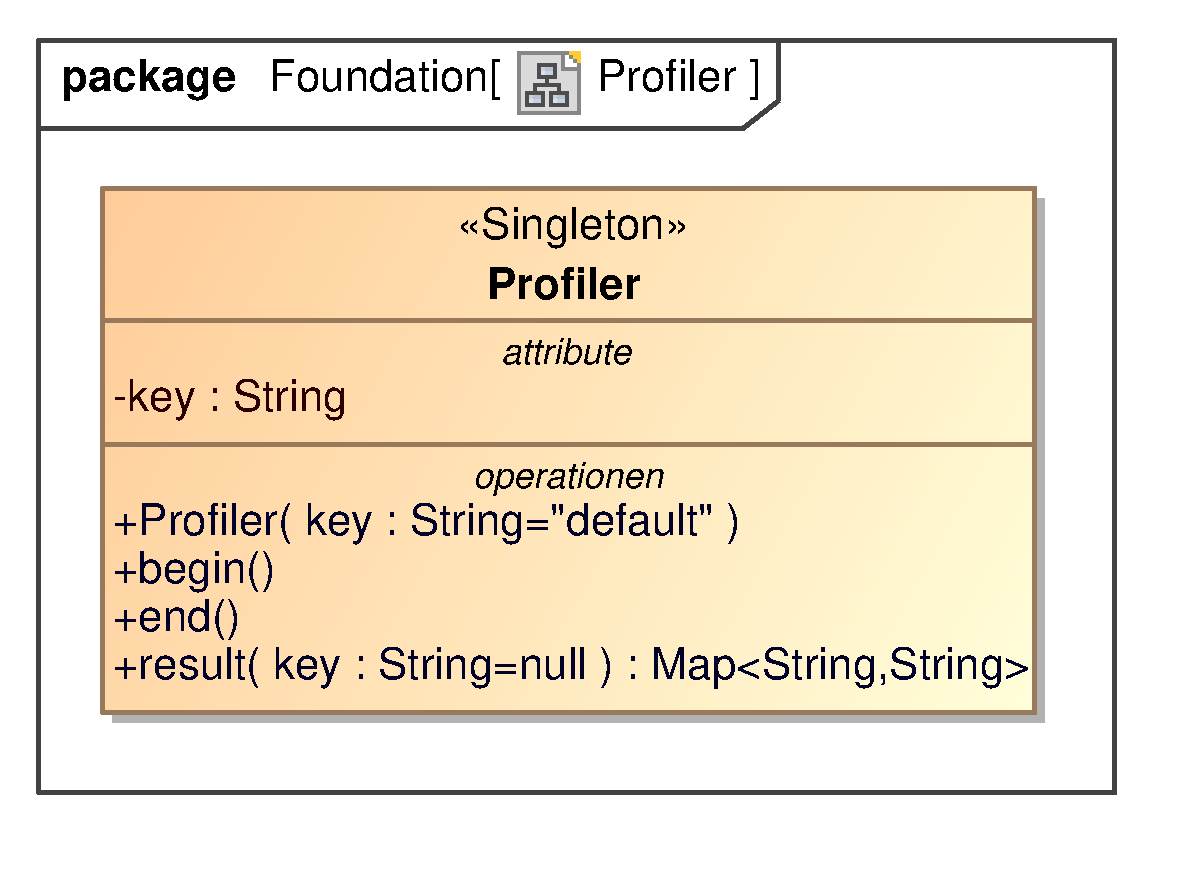
\includegraphics[width=0.75\textwidth]{gfx/MtGDeepAnalysis/Profiler.eps}
    \caption{Klassendiagramm Foundation.Profiler}
    \label{fig:class:foundation.profiler}
\end{figure}

\begin{description}
    \item[Profiler(key)] \hfill \\
    Erstellt eine neue \verb|Profiler| Instanz mit dem Schlüssel \verb|key| falls noch keine Vorhanden ist
    
    \item[begin()] \hfill \\
    Startet den Profiler
    
    \item[end()] \hfill \\
    Beendet der Profiler und speichert die gemessene Laufzeit und Speicherverbrauch
    
    \item[result(key : String)] \hfill \\
    Gibt das Ergebnis für des Profilers \verb|key| zurück
\end{description}

%%%%%%%%%%%%%%
%% Scrapers %%
%%%%%%%%%%%%%%
\subsubsection{Scrapers.Spider}
Die Klasse \verb|Scrapers.Spider| hat die folgenden Schnittstellen:

\begin{figure}[H]
    \myfloatalign
    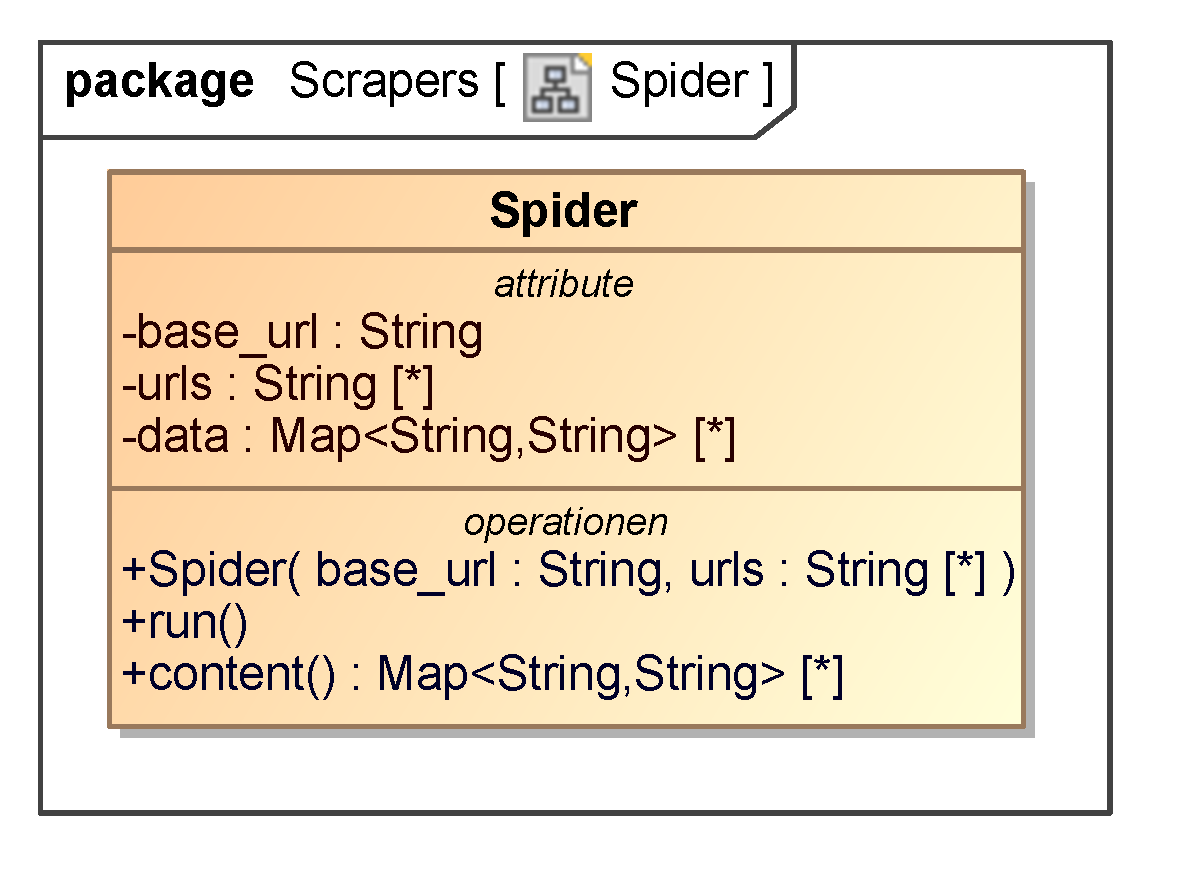
\includegraphics[width=0.65\textwidth]{gfx/MtGDeepAnalysis/Spider.eps}
    \caption{Klassendiagramm Scrapers.Spider}
    \label{fig:class:Scrapers.Spider}
\end{figure}

\begin{description}
    \item[Spider(base\_url, urls)] \hfill \\
    Initiert die Spider Klasse
    
    \item[run] \hfill \\
    Lädt die Decks von \verb|urls| und speichert diese
    
    \item[content()] \hfill \\
    Gibt die heruntergeladenen Decks zurück
\end{description}

\subsubsection{Scrapers.Decks}
Die Klasse \verb|Scrapers.Decks| hat die folgenden Schnittstellen:

\begin{figure}[H]
    \myfloatalign
    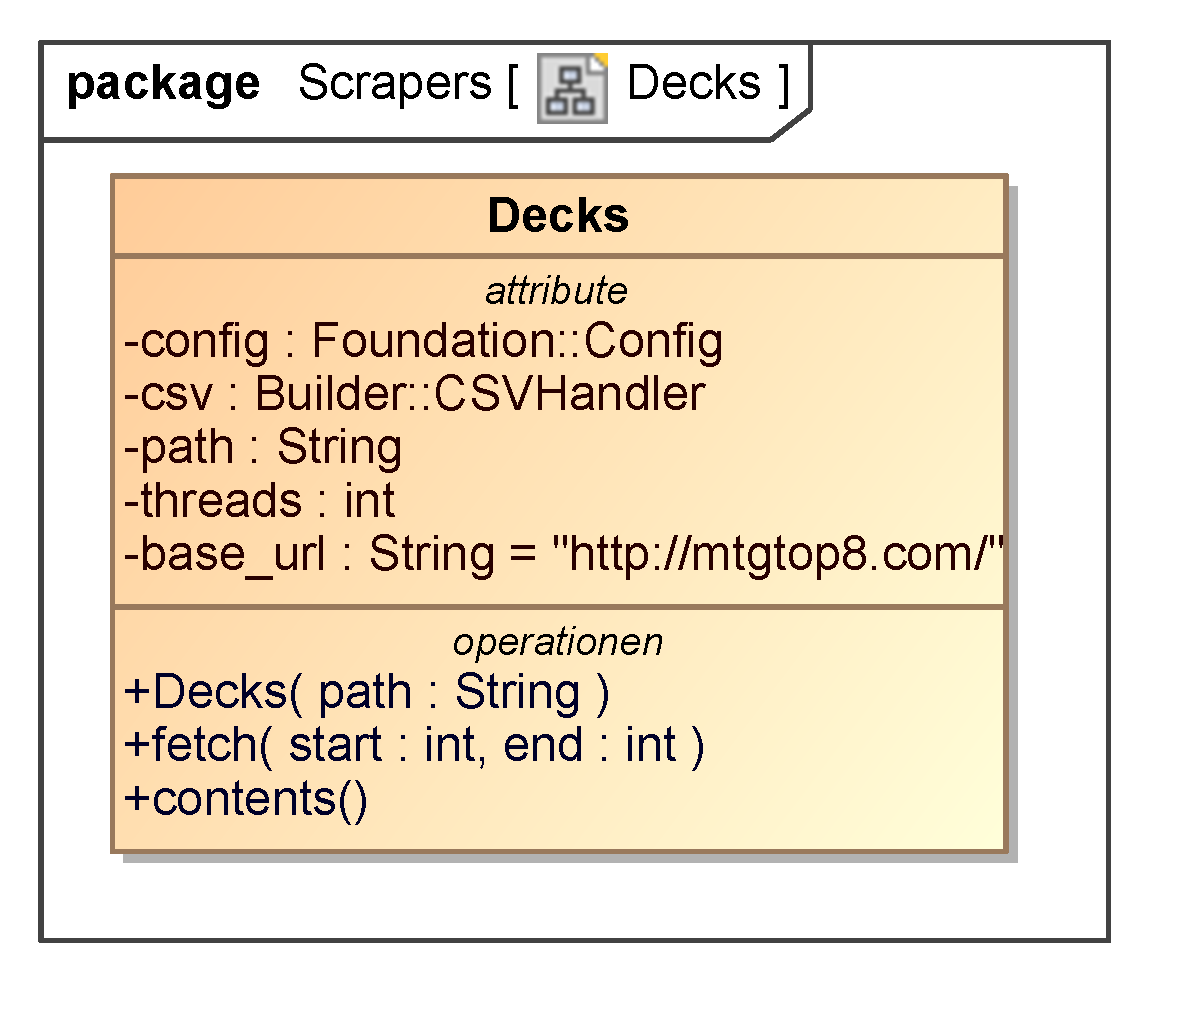
\includegraphics[width=0.65\textwidth]{gfx/MtGDeepAnalysis/Decks.eps}
    \caption{Klassendiagramm Scrapers.Decks}
    \label{fig:class:Scrapers.Decks}
\end{figure}

\begin{description}
    \item[Decks(path)] \hfill \\
    Initiert den CSVHandler mit \verb|path|
    
    \item[fetch(start, end)] \hfill \\
    Lädt die Decks per \verb|Spider| und speichert diese per \verb|CSVHandler| in einer \verb|decks.csv|
    
    \item[contents()] \hfill \\
    Extrahiert die Karten aus den heruntergeladenen Decks und speichert diese in eigener \ac{CSV} Datei
\end{description}

%%%%%%%%%%%%%%%%%%%%%
%% Transformations %%
%%%%%%%%%%%%%%%%%%%%%
\subsubsection{Transformations.Cards}
Die Klasse \verb|Transformations.Cards| hat die folgenden Schnittstellen:

\begin{figure}[H]
    \myfloatalign
    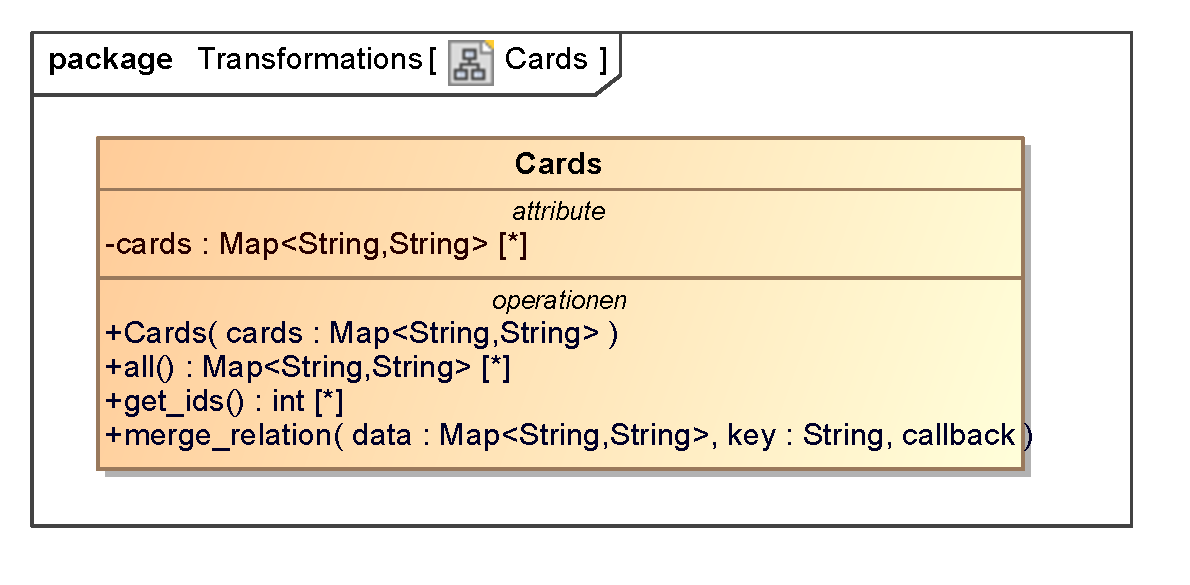
\includegraphics[width=0.75\textwidth]{gfx/MtGDeepAnalysis/Card_Transformations.eps}
    \caption{Klassendiagramm Transformations.Cards}
    \label{fig:class:transformations.cards}
\end{figure}

\begin{description}
    \item[constructor(cards)] \hfill \\
    Speichert die Karten \verb|cards|
    
    \item[all()] \hfill \\
    Ausgabe aller Karten
    
    \item[get\_ids()] \hfill \\
    Gibt eine List von allen Karten-IDs zurück.
    
    \item[merge\_relation(data, key, callback)] \hfill \\
    Fügt die Daten einer Beziehung zu den Karten-Daten hinzu. Die Liste der Argumente befindet sich in \autoref{tab:transformations.cards.merge_relation}
\end{description}

\begin{table}[h]
    \caption{Transformations.Cards::merge\_relation(data : Dictionary[], key : string, callback : Closure)} 
    \myfloatalign
    \begin{tabularx}{\textwidth}{lX}
        \toprule 
        \tableheadline{Eingabe} & \tableheadline{Beschreibung} \\ 
        \midrule 
        \verb|data : Map<String,String>| & Daten der Verknüpfung \\
        \verb|key : string| & Name unter dem die Verknüpfung in den Karten-Daten verfügbar sein soll \\
        \verb|callback : Closure| & Funktion, um Elemente der Verknpüfung zu bearbeiten bevor diese zu den Karten-Daten hinzugefügt werden \\
        \bottomrule 
    \end{tabularx}
    \label{tab:transformations.cards.merge_relation}
\end{table}


%%%%%%%%%%%%%
%% Builder %%
%%%%%%%%%%%%%

\subsubsection{Builder.Builder}
Die Klasse \verb|Builder.Builder| hat die folgenden Schnittstellen:

\begin{figure}[H]
    \myfloatalign
    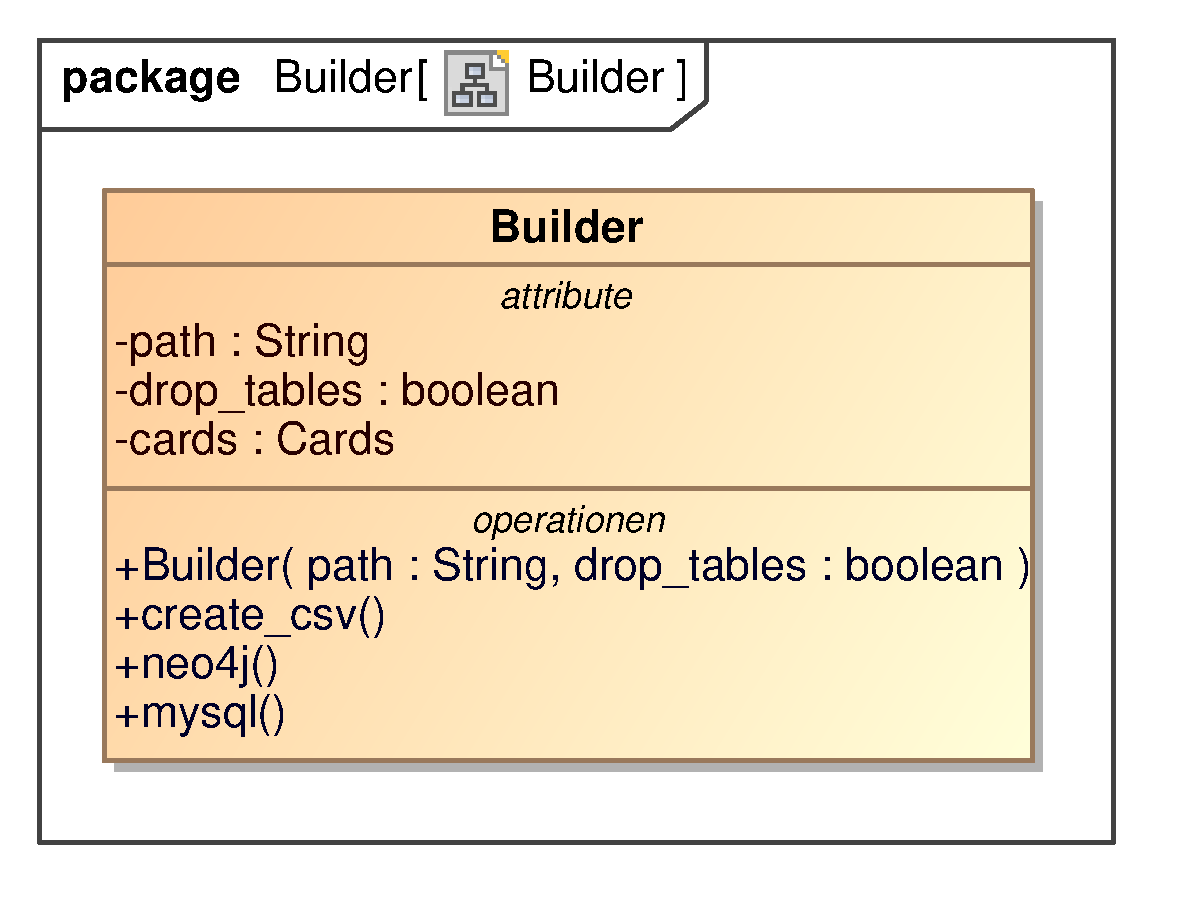
\includegraphics[width=0.65\textwidth]{gfx/MtGDeepAnalysis/Builder.eps}
    \caption{Klassendiagramm Builder.Builder}
    \label{fig:class:builder.builder}
\end{figure}

\begin{description}
    \item[constructor(path, drop\_tables)] \hfill \\
    Einrichten der Datenstruktur \verb|Cards|, speicher des Pfades zur \ac{JSON}-Datei, welche die Karten-Daten enthält
    
    \item[create\_csv()] \hfill \\
    Lädt die Kartendaten aus der \ac{JSON}-Datei und speichert die aufbereiteten Ergebnisse in \ac{CSV}-Dateien
    
    \item[neo4j()] \hfill \\
    Erstellt und befüllt die Neo4j Datenbank mit den Daten aus den \ac{CSV}-Dateien. Löscht alte Daten falls \verb|drop_tables = True|
    
    \item[mysql()] \hfill \\
    Erstellt und befüllt die MySQL Datenbank mit den Daten aus den \ac{CSV}-Dateien. Löscht alte Daten falls \verb|drop_tables = True|
\end{description}

\subsubsection{Builder.CSVHandler}
Die Klasse \verb|Builder.CSVHandler| hat die folgenden Schnittstellen:

\begin{figure}[H]
    \myfloatalign
    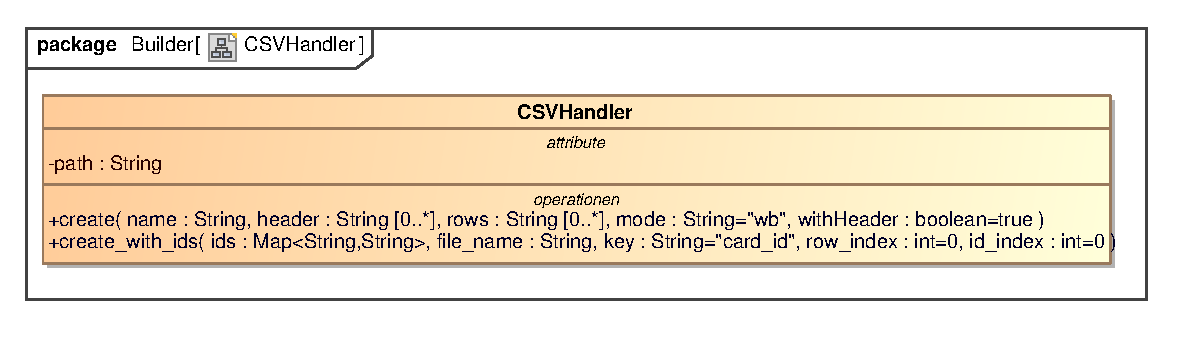
\includegraphics[width=\textwidth]{gfx/MtGDeepAnalysis/CSVHandler.eps}
    \caption{Klassendiagramm Builder.CSVHandler}
    \label{fig:class:builder.CSVHandler}
\end{figure}

\begin{description}
    \item[CSVHandler(path)] \hfill \\
    Speichert Pfadangabe
    
    \item[create(name, header, rows, mode="wb", withHeader=True)] \hfill \\
    Erstellt eine \ac{CSV}-Datei mit dem Namen \verb|name| und dem Header \verb|header| und befüllt diese mit den Reihen \verb|rows|. Mit \verb|mode| kann der Schreibmodus \emph{(überschreiben, anhängen)} angegeben werden und mit \verb|withHeader| ob der \verb|header| hinzugefügt werden soll.
    
    \item[create\_with\_ids(ids, file\_name, key="card\_id", row\_index=0, id\_index=0)] \hfill \\
    Erstellt eine \ac{CSV}-Datei mit dem Namen \verb|file_name| welche die IDs vom Typ \verb|key| hat. \verb|row_index| gibt den Index der CSV Spalte an, die die ID erhält und \verb|id_index| den Index an dessen Stelle die ID sich in \verb|ids| befindet.
\end{description}

\subsubsection{Builder.Cards}
Die Klasse \verb|Builder.Cards| hat die folgenden Schnittstellen:

\begin{figure}[H]
    \myfloatalign
    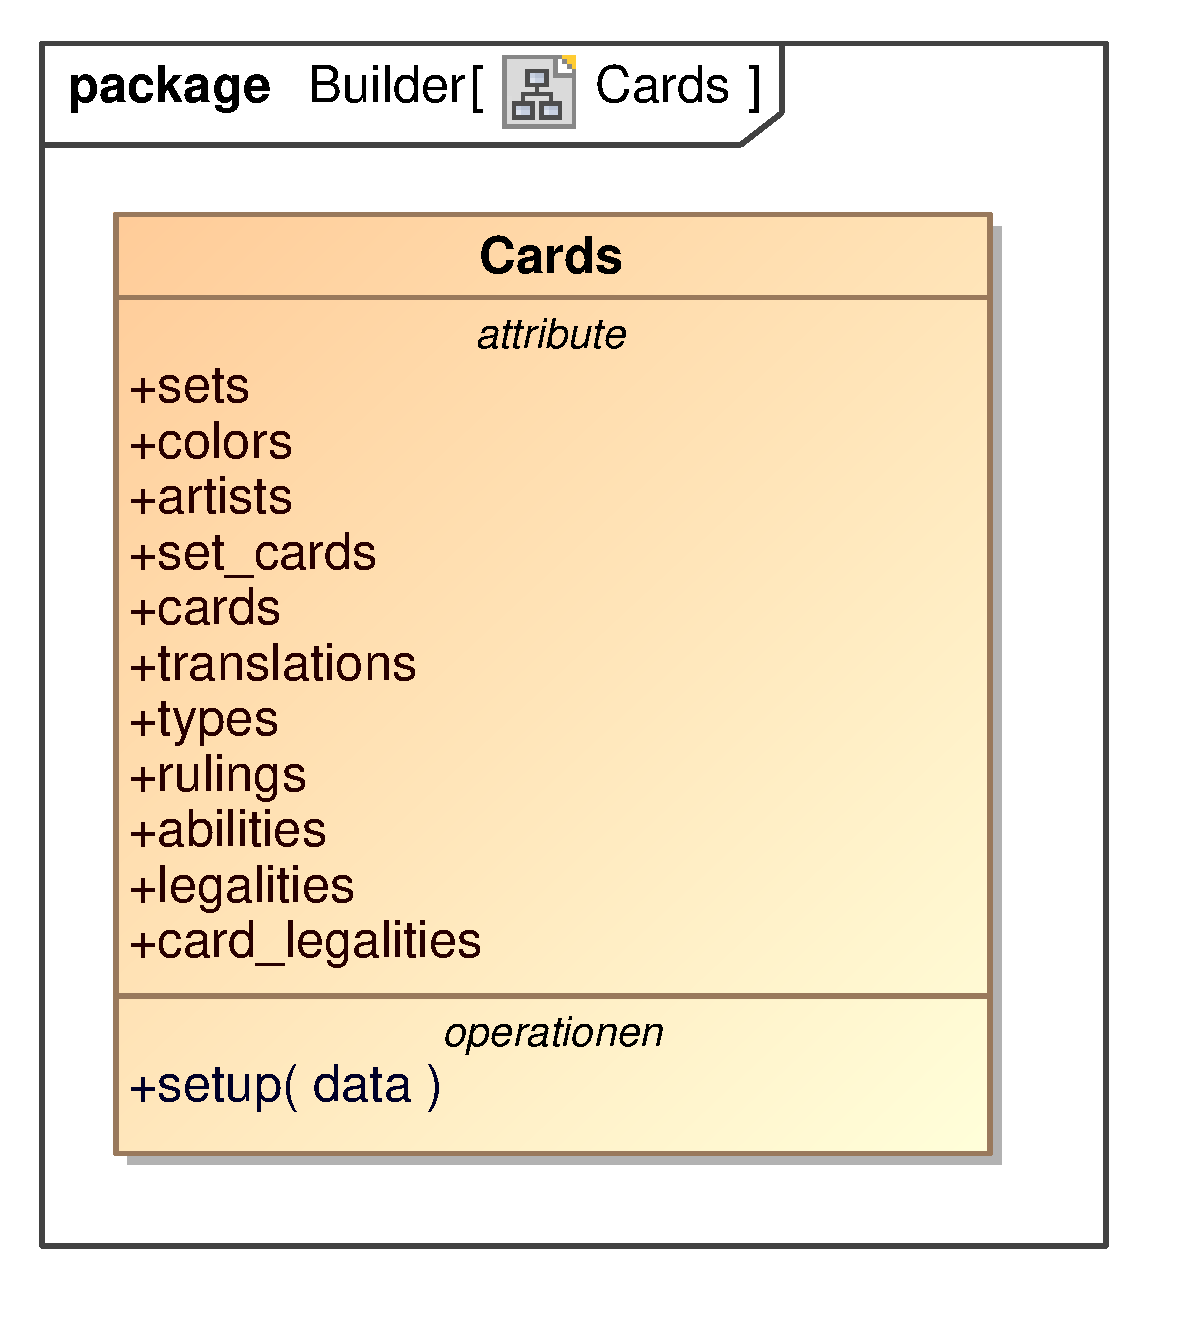
\includegraphics[width=0.5\textwidth]{gfx/MtGDeepAnalysis/Cards.eps}
    \caption{Klassendiagramm Builder.Cards}
    \label{fig:class:builder.cards}
\end{figure}

\begin{description}
    \item[Cards()] \hfill \\
    Erstelle Listen und Daten-Container.
    
    \item[setup(data)] \hfill \\
    Bearbeitet Kartendaten \verb|data|, so dass diese als \ac{CSV}-Dateien gespeichert werden können für den späteren Datenbank-Import.
\end{description}



\subsubsection{Builder.Tournaments}
Die Klasse \verb|Builder.Tournaments| hat die folgenden Schnittstellen:

\begin{figure}[H]
    \myfloatalign
    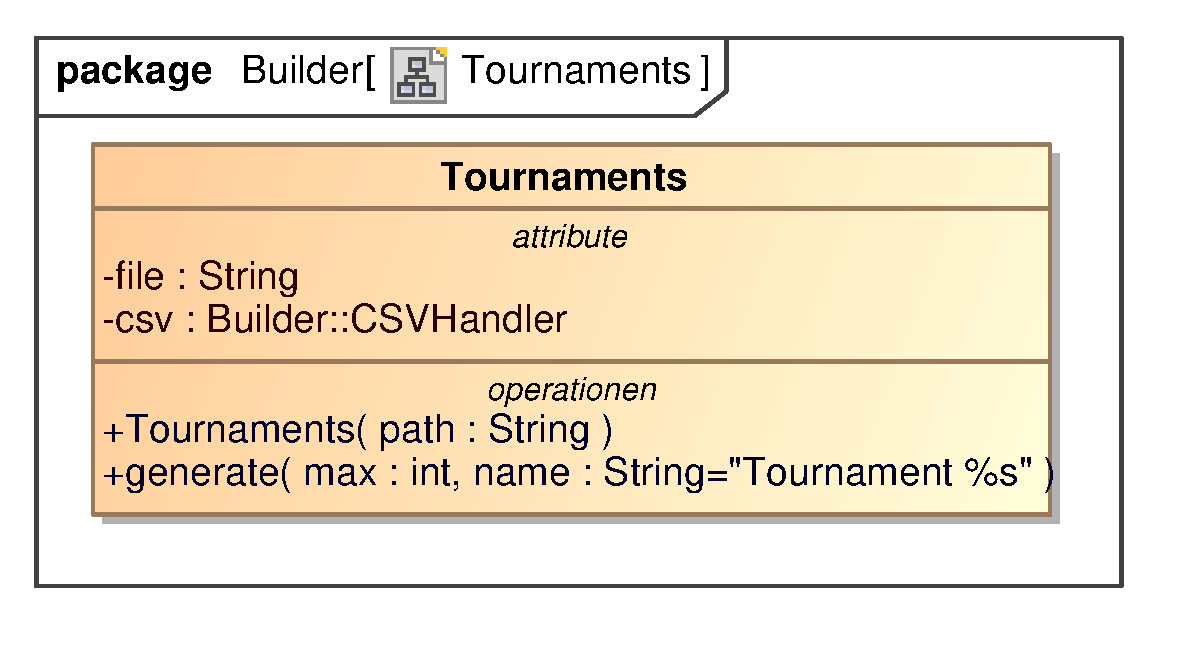
\includegraphics[width=0.65\textwidth]{gfx/MtGDeepAnalysis/Tournaments.eps}
    \caption{Klassendiagramm Builder.Tournaments}
    \label{fig:class:builder.Tournaments}
\end{figure}

\begin{description}
    \item[Tournaments(path)] \hfill \\
      Initiiert den \verb|CSVHandler| mit \verb|path|
     
    \item[generate(max, name="Tournament \%s")] \hfill \\
    Generiere \verb|max| Turniere mit den Namen \verb|name|
\end{description}

\subsubsection{Builder.Scaling}
Die Klasse \verb|Builder.Scaling| hat die folgenden Schnittstellen:

\begin{figure}[H]
    \myfloatalign
    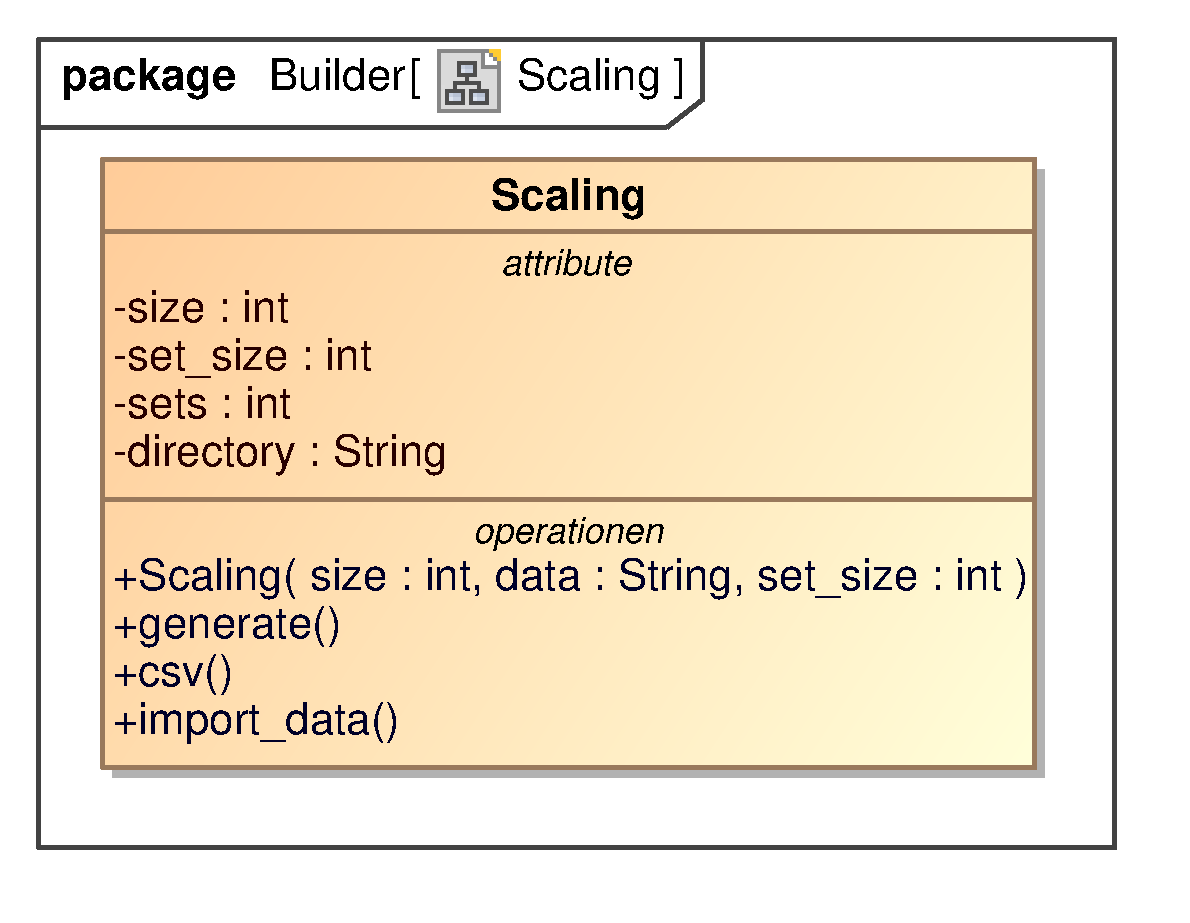
\includegraphics[width=0.65\textwidth]{gfx/MtGDeepAnalysis/Scaling.eps}
    \caption{Klassendiagramm Builder.Scaling}
    \label{fig:class:builder.Scaling}
\end{figure}

\begin{description}
    \item[Scaling(size, data, set\_size=250)] \hfill \\
    Berechne die Anzahl der zu generierenden Sets anhand von \verb|size| und \verb|set_size| und erstelle die nötigen Verzeichnisse in \verb|data|.
    
    \item[generate()] \hfill \\
    Generiere Dummy-Data und speichere diese als \ac{JSON} Dateien
    
    \item[csv()] \hfill \\
    Lade Dummy-Data aus \ac{JSON} Dateien und speichere diese als \ac{CSV} Dateien, sodass sie von der Datenbank importiert werden können
    
    \item[import\_data()] \hfill \\
    Importiere die generierten \ac{CSV} in die beiden Datenbanken
\end{description}


%%%%%%%%%%%%%%%%%%%%%%
%% Builder.Handlers %%
%%%%%%%%%%%%%%%%%%%%%%
\subsubsection{Builder.Handlers.MySQLBuilder}
Die Klasse \verb|Builder.Handlers.MySQLBuilder| hat die folgenden Schnittstellen:

\begin{figure}[H]
    \myfloatalign
    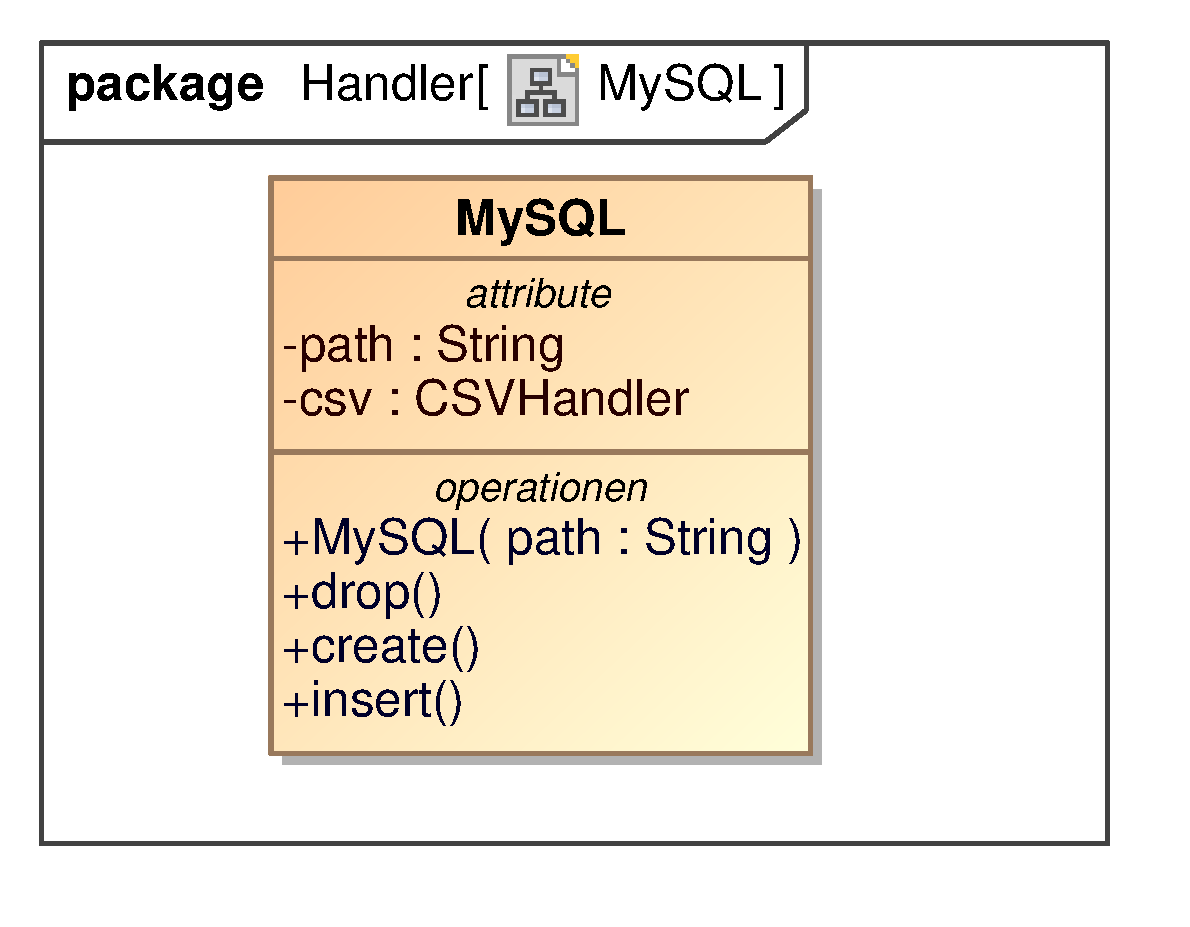
\includegraphics[width=0.5\textwidth]{gfx/MtGDeepAnalysis/MySQL.eps}
    \caption{Klassendiagramm Builder.Handlers.MySQLBuilder}
    \label{fig:class:builder.handlers.mysqlbuilder}
\end{figure}

\begin{description}
    \item[MySQL(path)] \hfill \\
    Initiiere den \verb|CSVHandler| mit \verb|path| und baue die Datenbankverbindung auf.
    
    \item[drop()] \hfill \\
       Löscht Tabellen.
       
    \item[create()] \hfill \\
        Erstellt Tabellen.
        
    \item[insert()] \hfill \\
        Importiert Daten aus den \ac{CSV}-Dateien.
    
    \item[insert()] \hfill \\
        Importiert Dummy-Daten aus den erstellten Skalierungs-CSV-Dateien.
\end{description}


\subsubsection{Builder.Handlers.Neo4jBuilder}
Die Klasse \verb|Builder.Handlers.Neo4jBuilder| hat die folgenden Schnittstellen:

\begin{figure}[H]
    \myfloatalign
    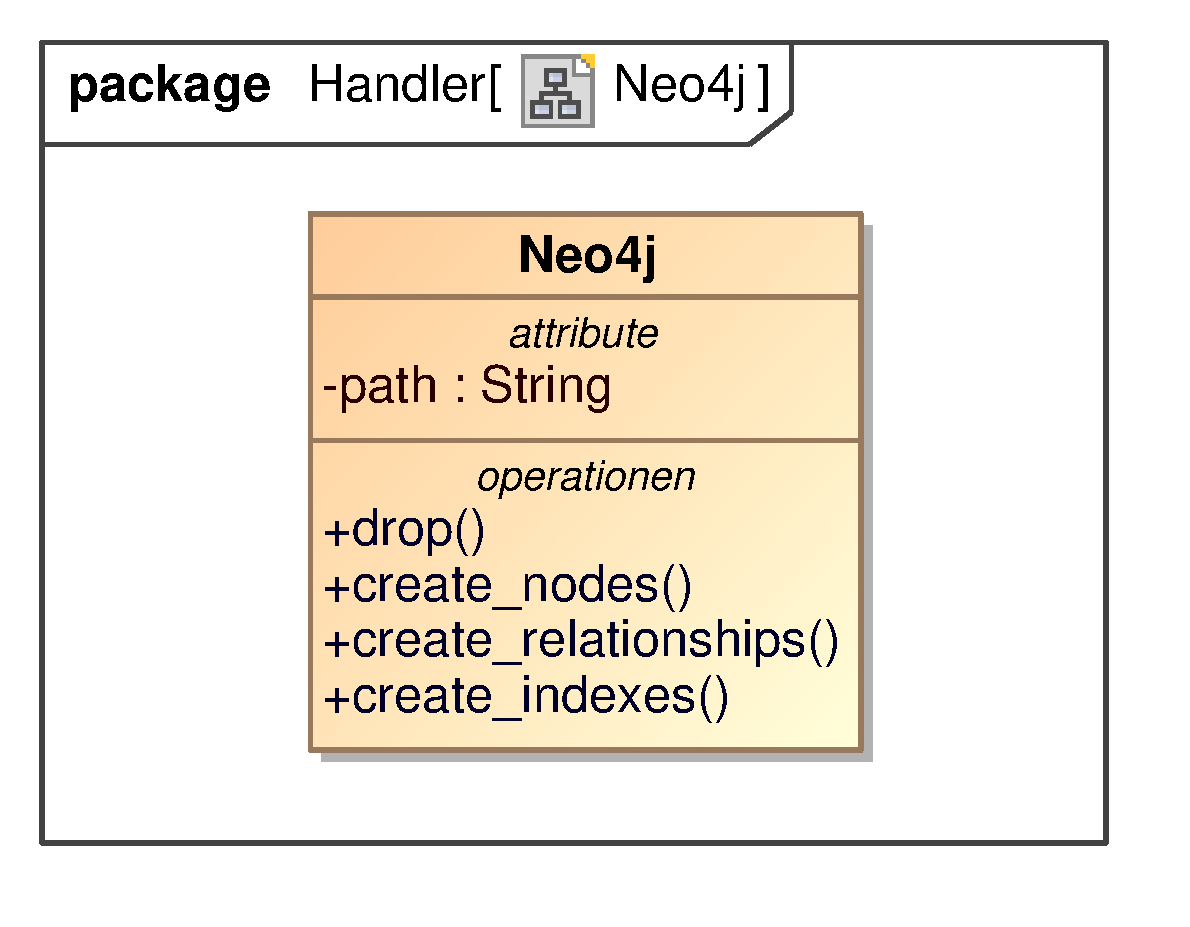
\includegraphics[width=0.5\textwidth]{gfx/MtGDeepAnalysis/Neo4j.eps}
    \caption{Klassendiagramm Builder.Handlers.Neo4jBuilder}
    \label{fig:class:builder.handlers.neo4jbuilder}
\end{figure}

\begin{description}
    \item[constructor(path)] \hfill \\
    Speichere die Pfadangabe \verb|path| zu den \ac{CSV}-Dateien und baue die Datenbankverbindung auf.
    
    \item[drop()] \hfill \\
    Löscht Datenbank.
    
    \item[create\_nodes()] \hfill \\
    Erstellt alle Knoten mit Daten aus den \ac{CSV}-Dateien.
    
    \item[create\_indexes()] \hfill \\
    Erstellt Indizes.
    
    \item[create\_relationships()] \hfill \\
    Erstellen Beziehungen zwischen Daten aus den \ac{CSV}-Dateien.
\end{description}

%%%%%%%%%%%%%%%%%
%% Tournaments %%
%%%%%%%%%%%%%%%%%

\subsubsection{Tournaments.Matches}
Die Klasse \verb|Tournaments.Matches| hat die folgenden Schnittstellen:

\begin{figure}[H]
    \myfloatalign
    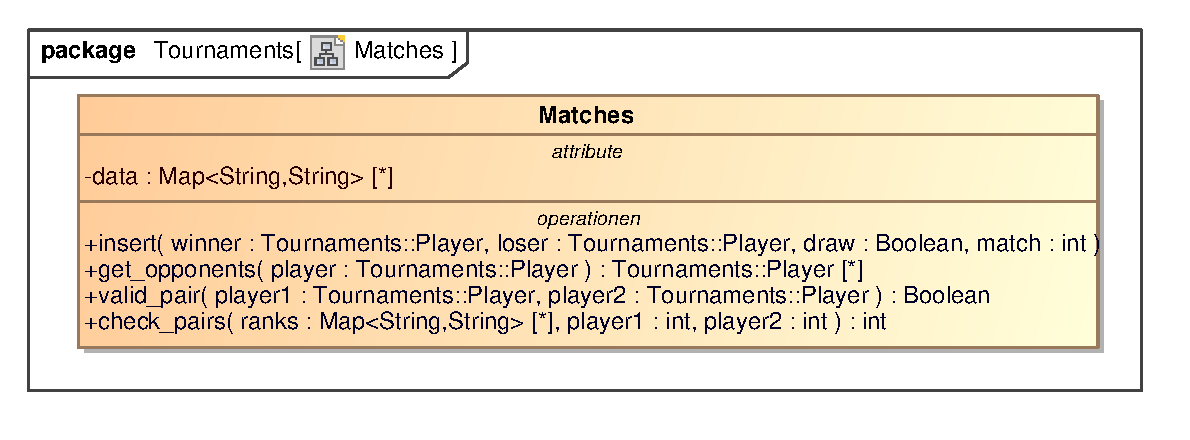
\includegraphics[width=0.95\textwidth]{gfx/MtGDeepAnalysis/Matches.eps}
    \caption{Klassendiagramm Tournaments.Matches}
    \label{fig:class:Tournaments.Matches}
\end{figure}

\begin{description}
    \item[insert(winner, loser, draw, match)] \hfill \\
    Hinzufügen eines neuen Matches
    
    \item[get\_opponents(player)] \hfill \\
    Gibt eine List mit allen bisherigen Gegnern von \verb|player| zurück.
    
    \item[valid\_pair(player1, player2)] \hfill \\
    Überprüft ob eine valide Paarung vorliegt, das heißt die beiden Spieler noch nicht gegeneinander gespielt haben.
    
    \item[check\_pairs(ranks, player1, player2)] \hfill \\
    Überprüft ob eine valide Paarung vorliegt, falls nicht suche rekursiv nach einem möglichen Spieler 2 für \verb|player1|
\end{description}

\subsubsection{Tournaments.Player}
Die Klasse \verb|Tournaments.Player| hat die folgenden Schnittstellen:

\begin{figure}[H]
    \myfloatalign
    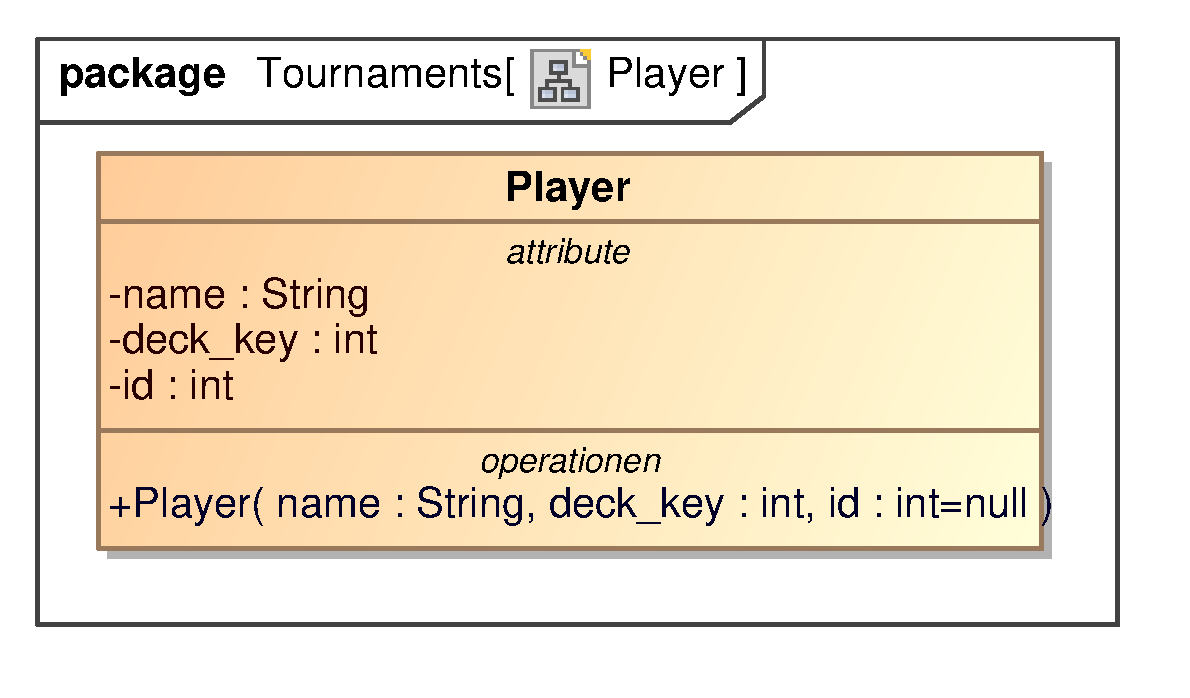
\includegraphics[width=0.65\textwidth]{gfx/MtGDeepAnalysis/Player.eps}
    \caption{Klassendiagramm Tournaments.Player}
    \label{fig:class:Tournaments.Player}
\end{figure}

\begin{description}
    \item[Player(name, deck\_key, id)] \hfill \\
    Anlegen eines Spielers \verb|name| mit der ID \verb|id| \emph{(falls vorhanden)} und dem Deck \verb|deck_key|
\end{description}

\subsubsection{Tournaments.Scoreboard}
Die Klasse \verb|Tournaments.Scoreboard| hat die folgenden Schnittstellen:

\begin{figure}[H]
    \myfloatalign
    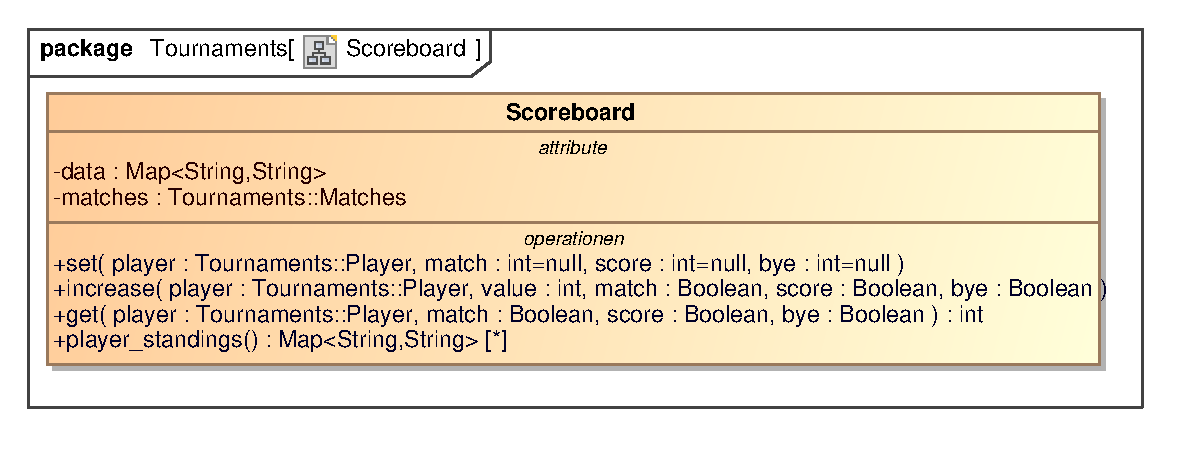
\includegraphics[width=\textwidth]{gfx/MtGDeepAnalysis/Scoreboard.eps}
    \caption{Klassendiagramm Tournaments.Scoreboard}
    \label{fig:class:Tournaments.Scoreboard}
\end{figure}

\begin{description}
    \item[(player, score, match, bye)] \hfill \\
    Setze das Ergebnis, Match oder den Bye eines Spielers \verb|player|
     
    \item[set(player, value, score, match, bye)] \hfill \\
    Erhöhe das Ergebnis, Match oder den Bye eines Spielers \verb|player| um \verb|value|
    
    \item[get(player, score, match, bye)] \hfill \\
    Gibt entweder das Ergebnis, Match oder den Bye eines Spielers \verb|player| zurück
    
    \item[player\_standings()] \hfill \\
    Gibt eine Liste der Spieler und ihrer Gewinn-Historie zurück, sortiert nach Siegen. Der erste Eintrag in der Liste sollte der Spieler an erster Stelle sein
\end{description}

\subsubsection{Tournaments.Tournament}
Die Klasse \verb|Tournaments.Tournament| hat die folgenden Schnittstellen:

\begin{figure}[H]
    \myfloatalign
    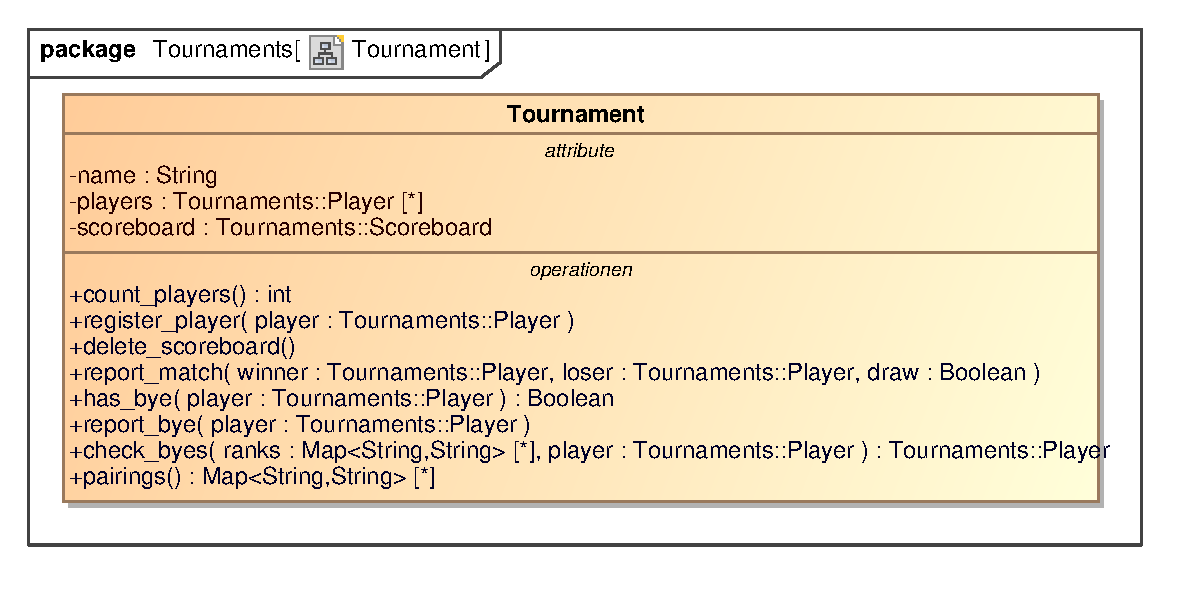
\includegraphics[width=\textwidth]{gfx/MtGDeepAnalysis/Tournament.eps}
    \caption{Klassendiagramm Tournaments.Tournament}
    \label{fig:class:Tournaments.Tournament}
\end{figure}

\begin{description}
    \item[count\_players()] \hfill \\
    Liefert die Anzahl der Spieler des Turniers
    
    \item[register\_player(player)] \hfill \\
    Fügt dem Turnier einen neuen Spieler hinzu
    
    \item[delete\_scoreboard()] \hfill \\
    Löscht Sie das Scoreboard und die Spielerliste
    
    \item[report\_match(winner, loser, draw)] \hfill \\
    Aufzeichnen der Ergebnisse eines einzelnen Spiels zwischen zwei Spielern.
    
    \item[has\_bye(player)] \hfill \\
    Prüft ob der Spieler Bye hat
    
    \item[report\_bye(player)] \hfill \\
    Füge dem Spieler Punkte für einen Bye hinzu
    
    \item[check\_byes(ranks, player)] \hfill \\
    Überprüfe ob der Spieler schon ein Bye hat, falls ja wird der erste Spieler zurückgegeben der noch kein Bye hat
    
    \item[pairings()] \hfill \\
    Gibt eine Liste von Spielernamen für die nächste Runde eines Spiels zurück. Unter der Annahme, dass es eine gerade Anzahl von registrierten Spielern gibt, erscheint jeder Spieler genau einmal in den Paarungen. Jeder Spieler wird mit einem anderen Spieler mit einem gleichen oder fast gleichen Gewinn Rekord gepaart.
\end{description}

%%%%%%%%%%%
%% Faker %%
%%%%%%%%%%%
\subsubsection{Faker.ManaCostProvider}
Die Klasse \verb|Faker.ManaCostProvider| hat die folgenden Schnittstellen:

\begin{figure}[H]
    \myfloatalign
    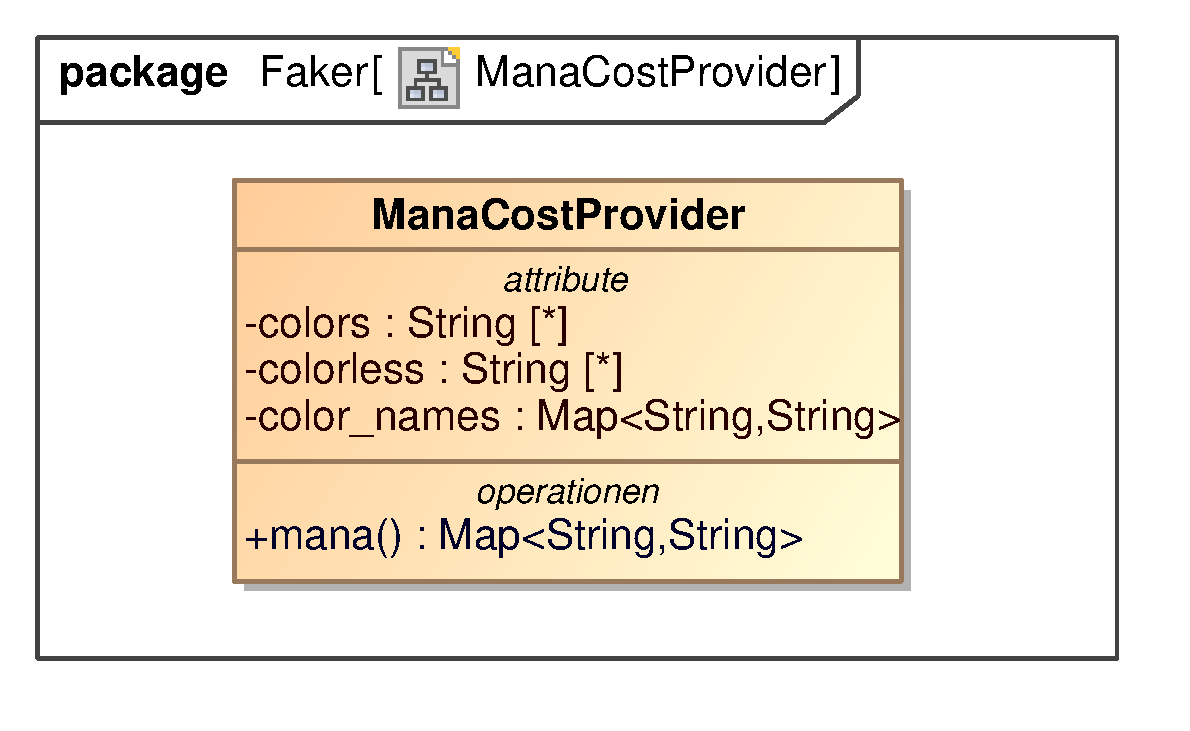
\includegraphics[width=0.6\textwidth]{gfx/MtGDeepAnalysis/ManaCostProvider.eps}
    \caption{Klassendiagramm Faker.ManaCostProvider}
    \label{fig:class:Faker.ManaCostProvider}
\end{figure}

\begin{description}
    \item[mana()] \hfill \\
    Liefert Mana-Kosten, Umgewandelte Manakosten und Farbe zurück
\end{description}

\subsubsection{Faker.TypeProvider}f
Die Klasse \verb|Faker.TypeProvider| hat die folgenden Schnittstellen:

\begin{figure}[H]
    \myfloatalign
    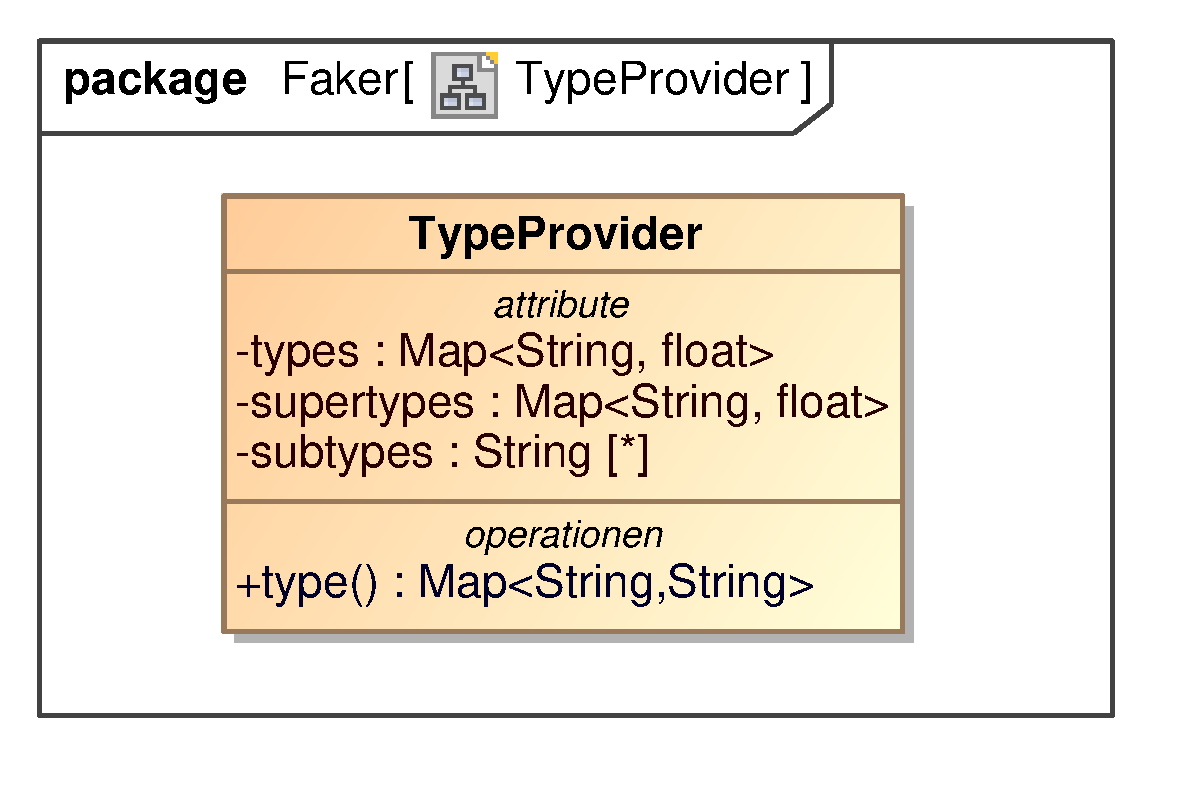
\includegraphics[width=0.6\textwidth]{gfx/MtGDeepAnalysis/TypeProvider.eps}
    \caption{Klassendiagramm Faker.TypeProvider}
    \label{fig:class:Faker.TypeProvider}
\end{figure}

\begin{description}
    \item[type()] \hfill \\
    Liefert Typ, Supertyp und Subtyp zurück
\end{description}

\subsubsection{Faker.CardProvider}
Die Klasse \verb|Faker.CardProvider| hat die folgenden Schnittstellen:

\begin{figure}[H]
    \myfloatalign
    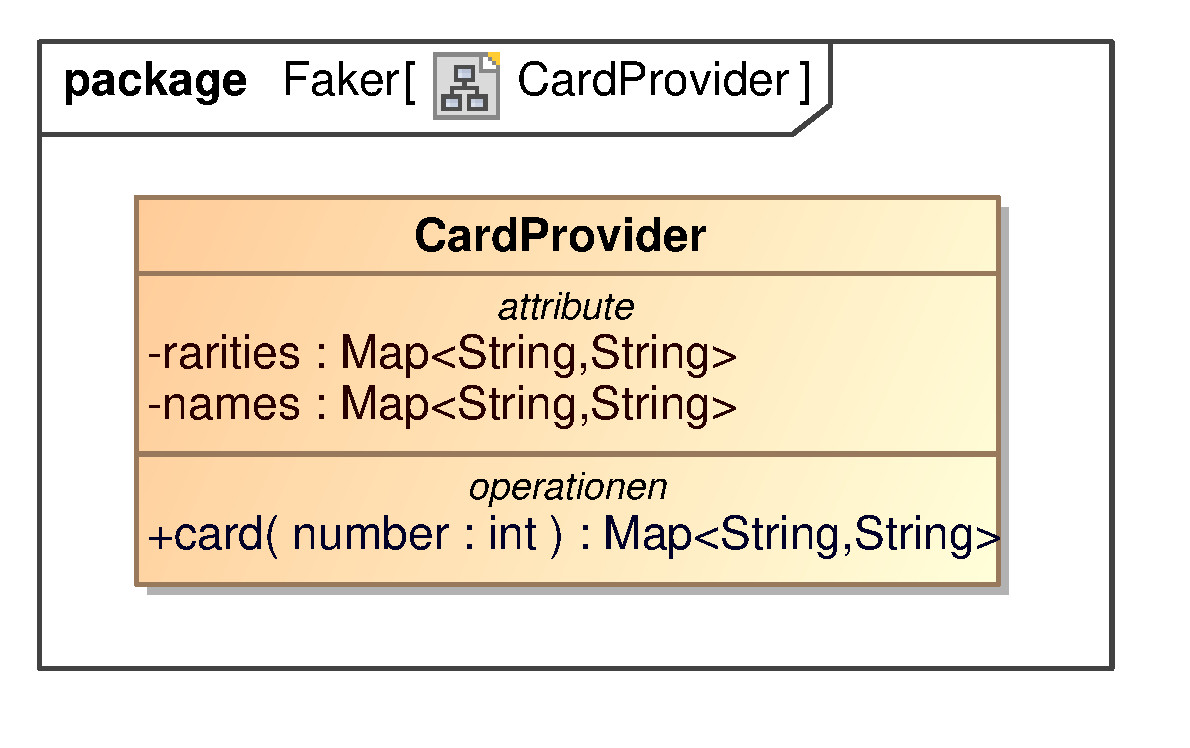
\includegraphics[width=0.6\textwidth]{gfx/MtGDeepAnalysis/CardProvider.eps}
    \caption{Klassendiagramm Faker.CardProvider}
    \label{fig:class:Faker.CardProvider}
\end{figure}

\begin{description}
    \item[card()] \hfill \\
    Liefert Daten zu einer Karte mit Nummber \verb|number| zurück
\end{description}

\subsubsection{Faker.SetProvider}
Die Klasse \verb|Faker.SetProvider| hat die folgenden Schnittstellen:

\begin{figure}[H]
    \myfloatalign
    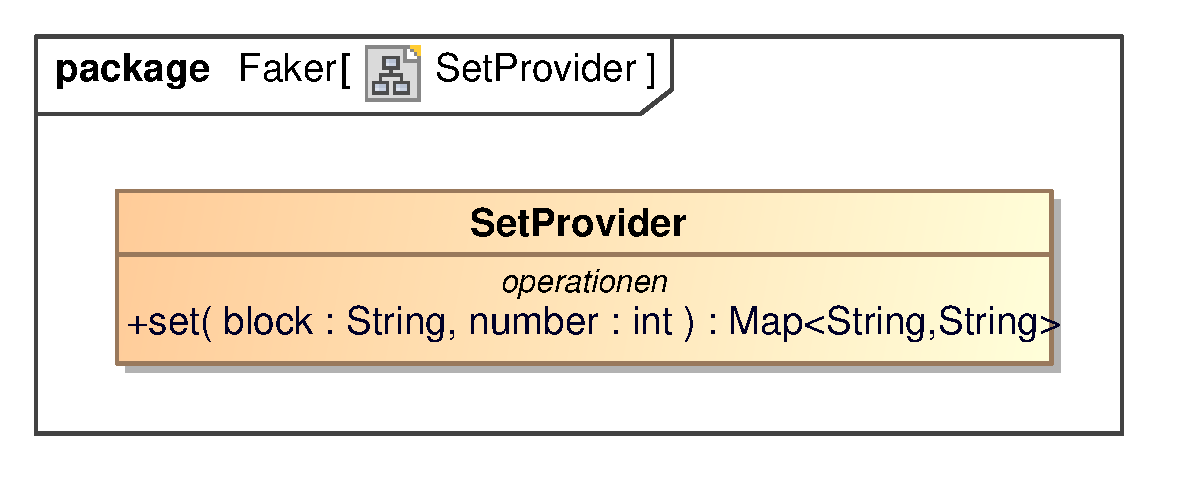
\includegraphics[width=0.6\textwidth]{gfx/MtGDeepAnalysis/SetProvider.eps}
    \caption{Klassendiagramm Faker.SetProvider}
    \label{fig:class:Faker.SetProvider}
\end{figure}

\begin{description}
    \item[card(block, number)] \hfill \\
    Liefert ein Set im \verb|block| Block mit \verb|number| Karten zurück
\end{description}


\subsection{Schnittstellenrealisierung}
%
% Schnittstellenrealisierung -> Interaktionsdiagramm
%
\subsubsection{Fetch} %TODO: Change title
Fetch decks from mtgtop8.com  %TODO: Change description

\begin{figure}[H]
    \myfloatalign
    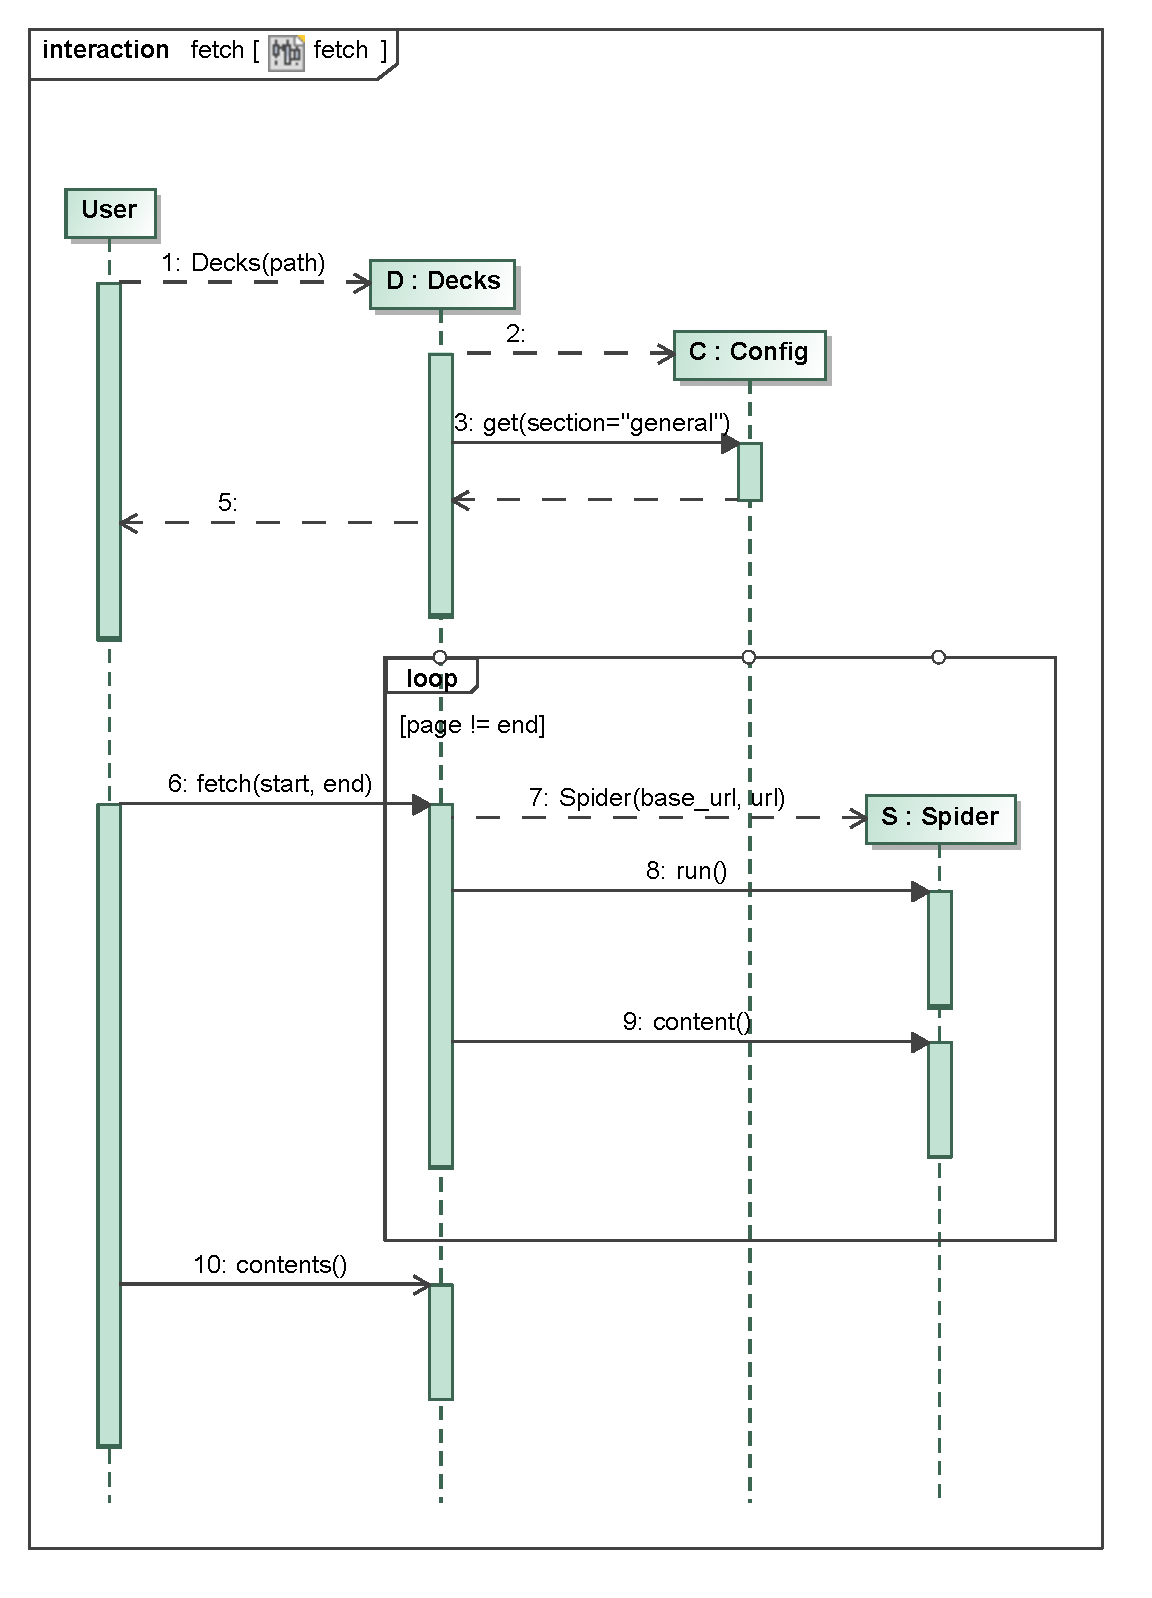
\includegraphics[width=\textwidth]{gfx/MtGDeepAnalysis/fetch.eps}
    \caption{Sequenzdiagramm Fetch} %TODO: Change caption
    \label{fig:seq:fetch}
\end{figure}

\subsubsection{Build} %TODO: Change title
Build mtgtop8 %TODO: Change description

\begin{figure}[H]
    \myfloatalign
    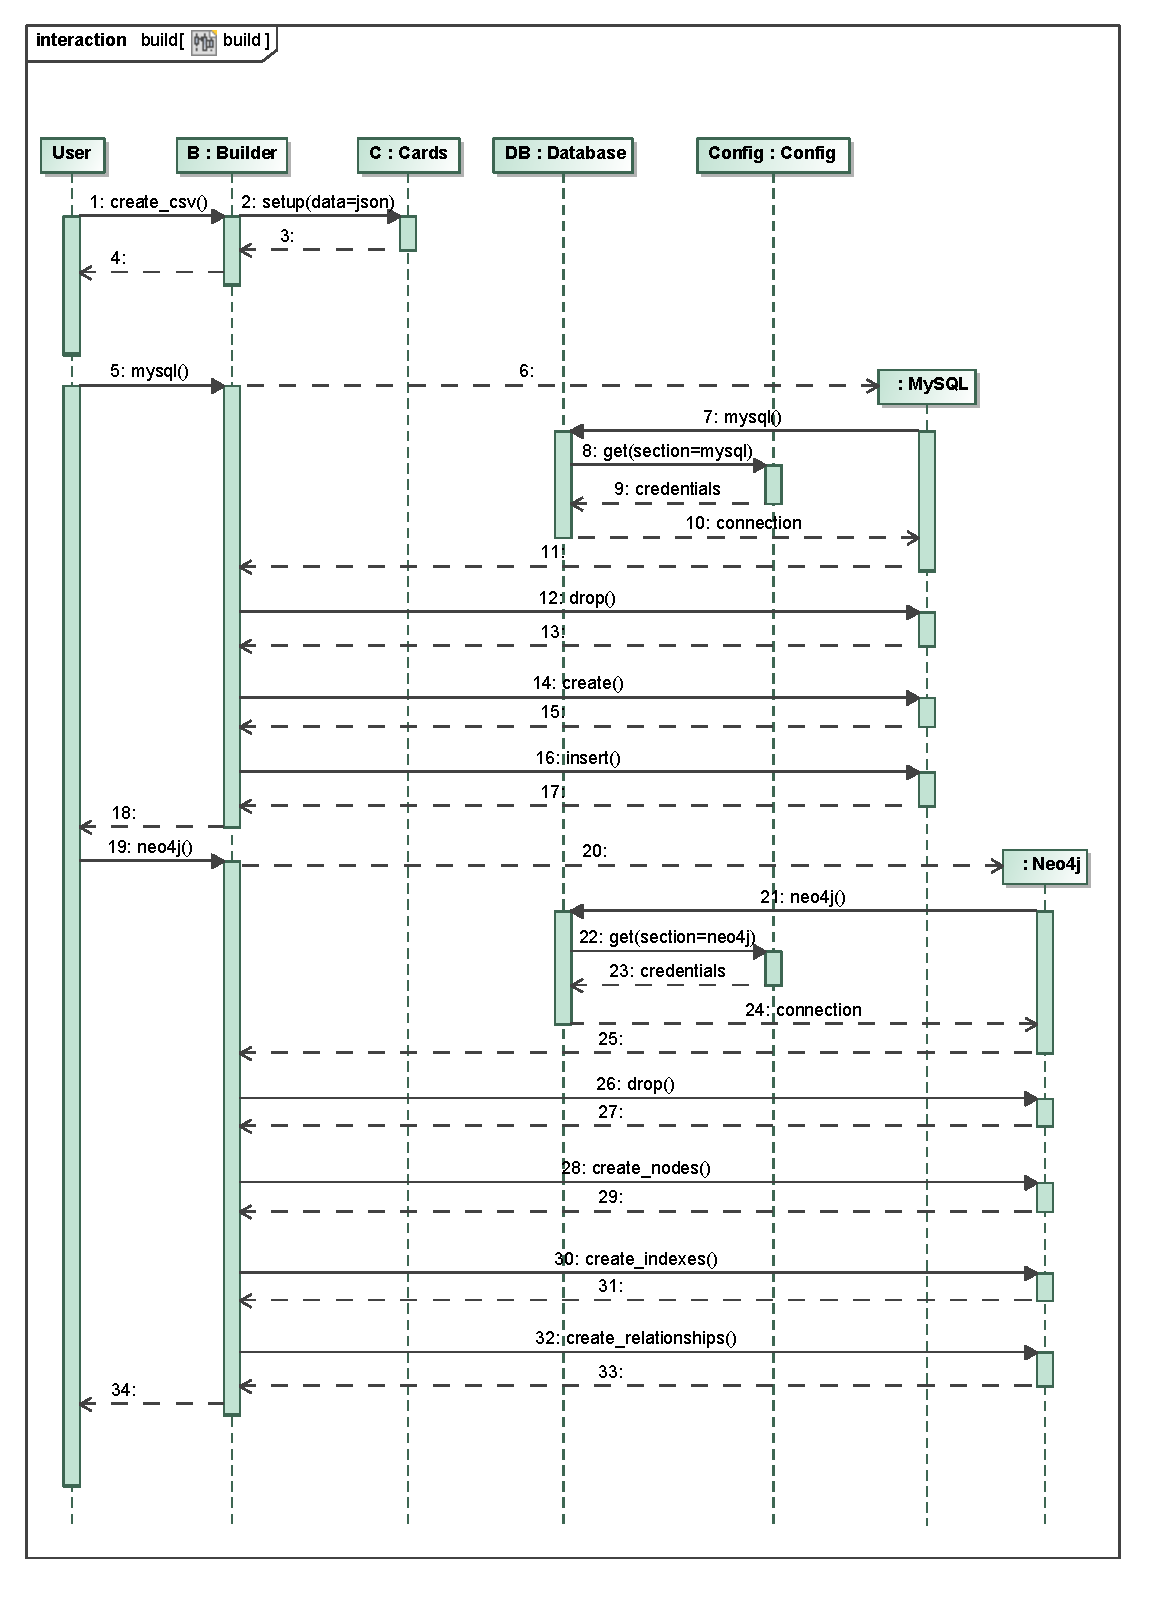
\includegraphics[width=\textwidth]{gfx/MtGDeepAnalysis/build.eps}
    \caption{Sequenzdiagramm build} %TODO: Change caption
    \label{fig:seq:build}
\end{figure}